
\chapter{Effective Data-preprocessing Pipelines in Supervised Learning}
\label{data-centric-chap:supervised}


To unleash the full potential of ML, data-centric AI focuses on shaping data according to the task and algorithm at hand.
With reference to the CRISP-DM process model,  \Cref{fig:data-analytics-pipeline} summarizes the stages involved and the corresponding problems in the literature.
% The decision making process has historically been key for the success of any organization or business activity.
% Lately, with the abundant presence of data, the learning process has become data-centric, i.e., to unleash the full potential of ML, data are shaped according to the task and algorithm at hand.
% and analyzed to be transformed into knowledge.
% As in CRISP-DM, along the way, data undergo several (sometimes necessary) pre-processing steps to finally be transformed into knowledge ---shown in \Cref{fig:data-analytics-pipeline}.
Firstly, data are extracted in a raw format from different sources and sifted out so that only a relevant subset is selected.
Next, during the pre-processing stage, the data pipeline selection and optimization (DPSO) \cite{Quemy19DOLAP} problem is tackled.
Once the data is transformed into the proper form, the modelling stage focuses on the combined algorithm selection and hyperparameter (CASH) optimization problem.
Finally, pipelines and algorithms
% (with different hyperparameters)
are evaluated over the dataset until an acceptable result is obtained.
%  --- \textit{ML model}.
% Despite the literature on data-centric AI, there are no universal well-defined practices for addressing DPSO  different steps, which translates to the data scientist manually configuring and parameterizing the transformations for each step until an optimal solution is found --- an optimal \textit{data pipeline}.



% this subset is pre-processed by selecting and optimizing a with series of transformations, i.e., data pipeline.
% this particular problem has been often referred to as the Data Pipeline Selection and Optimization problem (DPSO)~\cite{Quemy19DOLAP}, where a \textit{pipeline prototype} (sequence of transformations, e.g., missing value imputation followed by normalization) is fed to an optimizer and an optimal instance of the prototype, in the form of a \textit{pipeline} (sequence of operators, e.g., imputation by mean followed by min-max normalization) is found.

% Next, this subset is pre-processed with the aid of a data pipeline.
% Next, this subset is pre-processed and fed to an ML algorithm for it to be analyzed.
% The output of the analysis is then interpreted and the whole process iterates until the results obtained are satisfactory and significant for the decisions to be made.

% Unfortunately, this well-known process does not have universal well-defined practices for the different steps, which translates to the data scientist manually configuring and parameterizing the transformations for each step until an optimal solution is found --- an optimal \textit{data pipeline}.
% To this end, most of the time is spent on the heavily laborious work of pre-processing (i.e., 50-80\% of the time \cite{Munson09Pre}).
% , where the generated output is a \textit{pre-processing pipeline}.
% Once the data is transformed into the proper form, different ML algorithms with different hyperparameters are evaluated over the dataset until an acceptable result is obtained --- \textit{ML model}.
% This whole process requires expertise and is particularly challenging for novice, inexperienced data scientists for whom hand-tuning is no longer an option.

% Recent developments in algorithm configuration have raised the efficiency and effectiveness of automatic search, and therefore, for instance, AutoML is now considered a prominent technique for finding optimal models.
It is well-known that the whole process requires expertise and is particularly challenging.
Particularly, Data scientists spend most of their time on the heavily laborious work of pre-processing (i.e., around 50-80\% of the total \cite{Munson09Pre}).
Some AutoML frameworks \cite{auto_sklearn, mohr2018ml}, mix-in pre-processing during modelling optimization, but typically include very few transformations or do not consider all the necessary steps (e.g., imputation, rebalancing), thus in a way overlooking it.
Inspired from~\cite{Munoz09DOLAP}, we contend that there is need for more generic data-centric techniques, encompassing all the steps of data pre-processing \cite{Vaisman14Book}.
% ; from its inception via \textit{data extraction}, to the intermediate phase of \textit{data transformation}, up to the final phase, when data reaches its destination, via \textit{data loading}.
Assistance is required in every phase~\cite{Bilalli16IOTBD}.
% Yet, in a data analytics context, as in the case of this work, the critical automation challenge lies more on the \textit{data transformation} phase (see AutoETL and AutoML in Figure~\ref{fig:data-analytics-pipeline}), which is related to the pre-processing of the data.
% In the literature, this particular problem has been often referred to as the Data Pipeline Selection and Optimization problem (DPSO)~\cite{Quemy19DOLAP}, where a \textit{pipeline prototype} (sequence of transformations, e.g., missing value imputation followed by normalization) is fed to an optimizer and an optimal instance of the prototype, in the form of a \textit{pipeline} (sequence of operators, e.g., imputation by mean followed by min-max normalization) is found.
By considering pre-processing as an integral component of the learning process, and carefully selecting and optimizing data pipelines, it is easy to obtain results that go beyond the ones obtained by only optimizing ML algorithms.

\begin{figure*}[t]
    \centering
    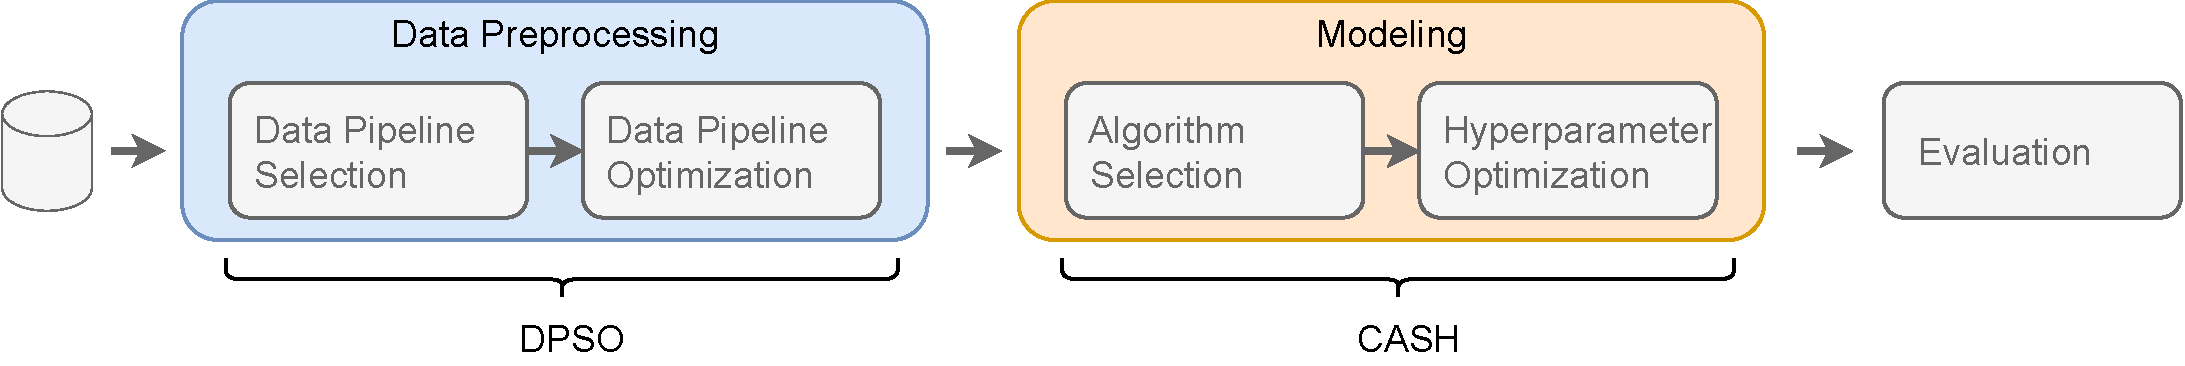
\includegraphics[width=1.0\textwidth]{chapters/data-centric/supervised/img/data-analytics-pipeline.pdf}
    \caption{Data analytics pipeline generation in a knowledge discovery process.}
    \label{fig:data-analytics-pipeline}
\end{figure*}

To briefly illustrate this, we perform an experiment on the well known \texttt{bank-marketing}\footnote{\url{https://archive.ics.uci.edu/ml/datasets/Bank+Marketing}} dataset, using HyperOpt~\cite{HyperOptICML13} as an AutoML approach to optimize the parameters of three different ML algorithms, namely Naive Bayes (NB), K-Nearest Neighbor (KNN), and Random Forest (RF).
We provide an initial budget of 50 iterations for optimizing the hyper-parameters of the algorithms, and after the 50th iteration, we fix the algorithm configuration to the best one achieved so far and start optimizing the pre-processing pipeline\footnote{This order is used only for the sake of illustration.}.
In \Cref{fig:pre-processing-impact}, the ratio of the change in terms of predictive accuracy (i.e., ratio of the accuracy obtained after the i-th iteration to the baseline/default accuracy) is plotted against the number of different configurations visited by HyperOpt (i.e., iterations).
Observe that after the 11th iteration for NB and KNN, and after the 26th iteration for RF, the lines remain flat.
That is, from there on, no improvement is achieved by optimizing the hyper-parameters of the algorithms until the 50th iteration is reached. At this point, a sudden jump is observed and the results start to improve again, going clearly beyond the ones obtained before, thanks to the optimizations performed now over the pre-processing pipeline.

\begin{figure}[t]
    \centering
    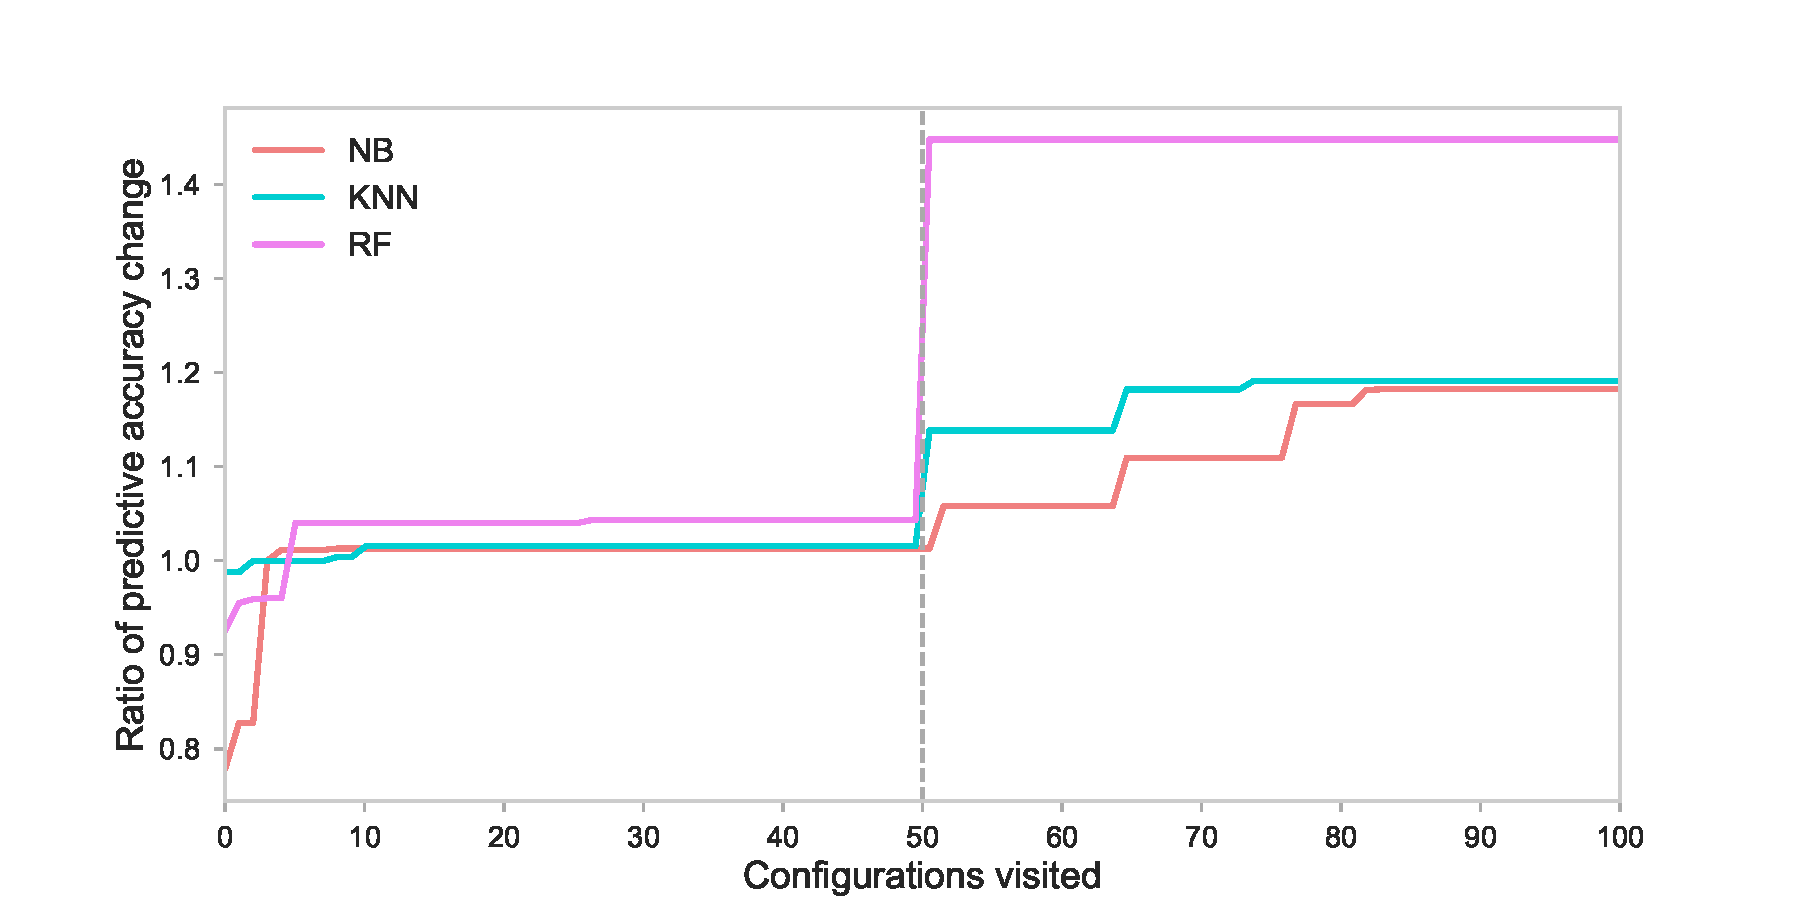
\includegraphics[width=0.7\textwidth]{chapters/data-centric/supervised/img/pre-processing-impact.pdf}
    \caption{Evolution of predictive accuracy during the optimization process. The first 50 configurations optimize only the hyper-parameters and after the 50th configuration, the pre-processing pipeline is optimized instead.}
    \label{fig:pre-processing-impact}
\end{figure}

\paragraph{Challenges} Including pre-processing in the learning process heavily increases the search space, making the problem much harder.
DPSO entails two challenges that the data scientists have to undergo to find the most appropriate pipeline: (i) choose how to order the different pre-processing steps  (i.e., pipeline selection), and (ii) choose which transformations, with corresponding hyperparameters, should be adopted in the final implementation  (i.e., pipeline optimization).
Following the notation from \cite{Quemy20InfSystems}, we also distinguish between the fixed and ordered sequence of pre-processing steps, known as \textit{prototype}, and the optimized instantiation of each transformation (with their hyperparameters), known as \textit{executable pipeline}.


% Including the pre-processing in a free form in the optimization, heavily increases the search space, making the problem much harder.
% This is mitigated by creating a pre-processing pipeline prototype that fixes the order of transformations, leaving the freedom to only instantiate and parametrize them.
% Therefore, the challenges that the data scientists have to undergo to find the most appropriate pre-processing are: (i) how to order the transformations  (i.e., prototype construction), and (ii) which pre-processing operators to consider in the prototype (i.e., prototype instantiation) such that when optimizing the parameters, better results are obtained.
% Furthermore, this work extends \cite{Giovanelli2021DOLAP}, among others with, (i) a new meta-learning step to guide the instantiation of transformations where a model is learned to predict the operators for a given transformation (see Section~\ref{sec:meta-learning}),
% (ii) a set of rules extracted through the meta learning process that mitigate the cold start problem (see Example 8), (iii) a new cross validation to confirm the initial results (see Section~\ref{sec:rules-learned}),
% (iv) a new background section for AutoML and AutoETL (see Section~\ref{sec:background}), and (v) experiments over new datasets (see Section~\ref{sec:evaluation}). 


\paragraph{Contributions} The aim of this chapter is to study these two questions raised in order to propose a method for selecting effective pre-processing pipelines that, once optimized through some optimization technique (e.g., Bayesian optimization), improve the final result of the analysis.
To keep discussions and experiments simpler, we stick to supervised learning tasks.
The main contributions of this paper can be summarized as follows.
\begin{itemize}
    \item We empirically evaluate the impact of optimizing the exhaustive set of potential prototypes and find out that at least one different pipeline works best for each dataset and algorithm considered, hence showing that there is no universal pipeline that works best for all of them.
    \item We define a method that given an ML algorithm and a set of pre-processing transformations, is capable of generating the right order between transformations, obtaining effective pre-processing pipeline prototypes, which are then instantiated and further optimized via bayesian optimization.
    \item We suggest a meta-learning step, where the relationship between pre-processing transformation and dataset characteristics is learned in order to create rules that help with the initial instantiation of the pipeline prototypes.
    % \begin{itemize}
    %      \item We exemplify our meta-learning study generating simple but not obvious and effective rules for two kinds of transformations, namely, Feature Engineering and Rebalancing.
    % \end{itemize}
    \item We perform a comprehensive evaluation by comparing the performance of optimizing the pipelines generated following our method, and find out that:
    \begin{enumerate}
        \item with 24 times less time budget, our proposed pipelines obtain results whose median is above 90\% of the ones generated via exhaustive search.
        \item on average, in 73\% of the cases, splitting evenly the time budget between pre-processing and hyper-parametrisation outperforms the results of only optimizing the hyper-parameters of the ML algorithm.
    \end{enumerate}
\end{itemize}

The remaining of this paper is organized as follows:
% Section~\ref{sec:background} provides a brief background on AutoETL and AutoML.
\Cref{sec:relatedwork} discusses the related work,
\Cref{sec:methodology} presents our method of generating effective pipelines,
\Cref{sec:evaluation} provides an extensive evaluation of the pipelines created using our proposed method and, finally, \Cref{sec:conclusions} provides the conclusions and future work.

% \section{Background: AutoETL and AutoML}
% \label{sec:background}


% The abundance of data has led to data analytics being prevalent in many disciplines and domains, but since the number of its applications exceeds the number of qualified experts, more and more non-experts approach the task of data analytics. This has consequently led to the rise of off-the-shelf automated techniques that facilitate its application.
% AutoML is an umbrella term for automations mainly related to the ML algorithm, and it typically aims to tackle the challenge of Combined Algorithm Selection and Hyperparameter Optimization (CASH). Yet, there is also need for automation in the more generic aspects of ETL~\cite{Munoz09DOLAP}, which we coin as AutoETL. AutoETL encompasses various steps, however, in this work we focus on the phase that is related to the transformation (pre-processing) of the data, typically formalized as DPSO.

% CASH and DPSO can be treated as a single optimization problem ~\cite{auto_weka, auto_sklearn}. However, we consider them separately because this allows to, (i) reduce the search space and, (ii) to explicitly assign different optimization budgets and/or optimization techniques, depending on their respective impact to the final result of the analysis.
% Since these problems are similar, the methods initially employed in CASH have been recently considered to solve the DPSO problem too. Therefore, in the following we first delve into more details about CASH and then DPSO. In particular, we formalize them and discuss the methods they employ.

% \subsection{Combined Algorithm Selection and Hyper-parameter optimization (CASH)}

% The algorithm selection problem is known to exist for a long time and many approaches have been proposed to solve it~\cite{Serban13survey}. Recently, in the context of ML algorithms, the problem has been extended to include the optimization of the hyperparameters too, and thus has been formalized as follows~\cite{auto_weka}.

% Given:
% \begin{itemize}
%     \item A data-set $D$ divided into $D_{train}, D_{test}$;
%     \item A set of algorithms $\mathcal{A} = \{A^{1}, \dots , A^{k}\}$ with associated hyperparameter spaces $\Lambda^{1}, \dots, \Lambda^{k}$;
%     \item And a loss function $\mathcal{L}(A^{i}_\lambda,D_{train},D_{test})$;
% \end{itemize}
% we are searching for:
% \begin{equation}
%     A^{\ast}_{\lambda^{\ast}} \in \argmin\limits_{A^i \in \mathcal{A}, \lambda \in \Lambda^i} \mathcal{L}(A^i_\lambda,D_{train},D_{test}) \tag{CASH}
% \end{equation}

% The dataset $D$ is divided into $D_{train}$ and $D_{test}$, to build and to evaluate the overall performance, calculated through the loss function $\mathcal{L}$. The problem is set up as an optimization problem and, as such, the configuration space is assumed to be known in advance (the set of algorithms $\{A^{1}, \dots , A^{k}\}$ and the related hyper-parameter spaces $\{\Lambda^{1}, \dots, \Lambda^{k}\}$).
% The goal is then to find the best algorithm $A^{\ast}$ in the set of algorithms and its best hyperparameters $\lambda^{\ast}$ in the related hyperparameter space. 

% Many optimization techniques have been employed to solve the CASH problem and some of them are: Grid search\textcolor{red}{~\cite{montgomery2017design}}, Random search\textcolor{red}{~\cite{bergstra2012random}}, Simulating annealing\textcolor{red}{~\cite{van1987simulated}}, Genetic algorithms\textcolor{red}{~\cite{kramer2017genetic}}, Bayesian techniques\textcolor{red}{~\cite{gp_kernel}}, Bandit-based algorithms~\textcolor{red}{\cite{li2017hyperband}}.
% However, due to their promising results, Bayesian techniques are perhaps the most popular ones~\cite{zoller2019survey,autoMLsurveyQuanming}. We explore their details and specifically focus on one of their incarnation, the Sequential Model-Based Optimization (SMBO) algorithm~\cite{hutter2011sequential}.

% \paragraph{Sequential Model-Based Optimization (SMBO)}

% In an optimization problem, we are searching for the best solution among a set of feasible solutions. The latter can be formalized as follows:
% \begin{equation*}
%     \max_{x \in B} f ( x )
% \end{equation*}
% , where $B$ contains all the feasible solutions, or candidates, and it is typically d-dimensional ($B \subseteq \mathbb{R}^d$), where $d \in \mathbb{Z}$ and $d>1$. A specific solution $x \in B$ is evaluated through the function $f: \mathbb{R}^d \longrightarrow \mathbb{R}$, also called the objective function. In general, in these kinds of problems,~$f$~has no special structure like concavity or linearity that would make the optimization easier. In fact, it is considered as a ``black-box'' function, without any knowledge about its behaviour; being that it maps certain inputs, $x \in B$, to certain outputs, $f(x) \in \mathbb{R}$. The goal is then finding an $x$ that maximizes $f(x)$.
% The naive solution to the problem would be to systematically evaluate all possible candidates $x$ and choosing the one leading to the highest value of $f(x)$, aka \textit{exhaustive search}. Since this evaluates all the potential solutions, it guarantees that it always finds the best one. Nevertheless, generally, it cannot be applied to real problems due to the large number of candidate solutions to be explored, which dwell in a high-dimensional space, and too expensive objective functions. The result is that not all candidates can be evaluated and we have to find a way to wisely choose the most promising ones.
% Bayesian techniques are part of the family of ``surrogate methods'', which create a surrogate model to approximate the objective function and thus, choose a point in the search space where to evaluate the objective function~\cite{BayesianOptimizationBook}. In contrast to the other methods, they build such surrogate models through Bayesian statistics.

% In short, Bayesian techniques start by evaluating the objective function on an initial observation point of the search space, then the process becomes iterative: the surrogate model is constructed on the basis of the visited points and through an acquisition function --- the Bayesian interpretation of the surrogate, the candidate for the next observation is decided. The process ends when a termination condition is reached, generally expressed through a \textit{budget} represented in terms of the \textit{number of iterations} or \textit{execution time}. Given its iterative nature and the fundamental role of the model, this algorithm is called Sequential Model-Based Optimization~\citep{hutter2011sequential,hutter2009experimental}. 
% Variations of SMBO exist, depending on the method used to build the surrogate model (e.g., Gaussian Processes, Random Forest Regressions)~\cite{snoeck2012NIPS,Wistuba2018ML}.

% \subsection{Data Pipeline Selection and Optimization (DPSO)}

% DPSO was formalized for the first time in \cite{Quemy20InfSystems}, where some new concepts were introduced. For instance, a pre-processing \textit{pipeline prototype} or \textit{logical pipeline} is defined as a sequence of kinds of transformations, where each represents a logical concept that can be implemented/instantiated by one or more operators. The prototype thus, defines only the order between kinds of transformations, without specifying the concrete operators nor their parameters. Yet, the potential operators of each kind and their corresponding parameter search spaces need to be known in advance. Solving the DPSO problem translates to finding the right instantiation and configuration for each kind of transformation in the pipeline prototype (i.e., optimal operator and optimal parameter values), which is called pre-processing \textit{pipeline} or \textit{physical pipeline}. 

% Formally, given:
% \begin{itemize}
%     \item A data-set $D$ divided into $D_{train}, D_{test}$;
%     \item A data pipeline prototype $P$ with a configuration space  $\mathcal{P}$;
%     \item The algorithm $A$, for which the given pipeline $P$ transforms the data;
%     \item And a loss function $\mathcal{L}(P,A,D_{train},D_{test})$;
% \end{itemize}
% we are searching for:
% \begin{equation}
%     P^\ast \in \argmin_{P \in \mathcal{P}} \mathcal{L}(P,A,D_{train},D_{test}) \tag{DPSO}
% \end{equation}

% Notice that a prototype imposes an order between the kinds of transformations, but this is an additional problem that is not dealt within DPSO, since it is assumed to be given as part of the input. This is in fact a limitation of the current approaches in DPSO, in that the order of kinds of transformations are fixed a priori without sufficiently studying the potential effectiveness of different alternatives.

% \paragraph{SMBO as solver for DPSO}

% Since DPSO is formalized as an optimization problem, SMBO has been proposed as a valid solver\textcolor{red}{~\cite{hutter2011sequential}}. In the previous section, we saw the application of SMBO to CASH, but in fact the process of selecting the best algorithm, and its hyperparameters configuration, is identical to selecting the best operator for a transformation, and its parameter configuration. Yet, DPSO requires one more layer, in that transformations need to be chained together into a pipeline.
% To this end, given a pipeline prototype as input and a budget either in terms of time or number of iterations, SMBO can be configured to iterate over different configurations until a near to optimal physical pipeline is found. The objective function of the pipeline is however measured in the context of a given parametrised ML algorithm by applying the pipeline on a dataset, and measuring the performance of the ML algorithm (e.g., predictive accuracy) on the transformed output. In this context, by fixing the hyper-parameters of the ML algorithm to the default ones, the performance of the learner is set to measure the effectiveness of the considered data pipeline. 


\section{Data pre-processing pipeline generation}
\label{sec:methodology}

\begin{figure*}[t]
    \centering
    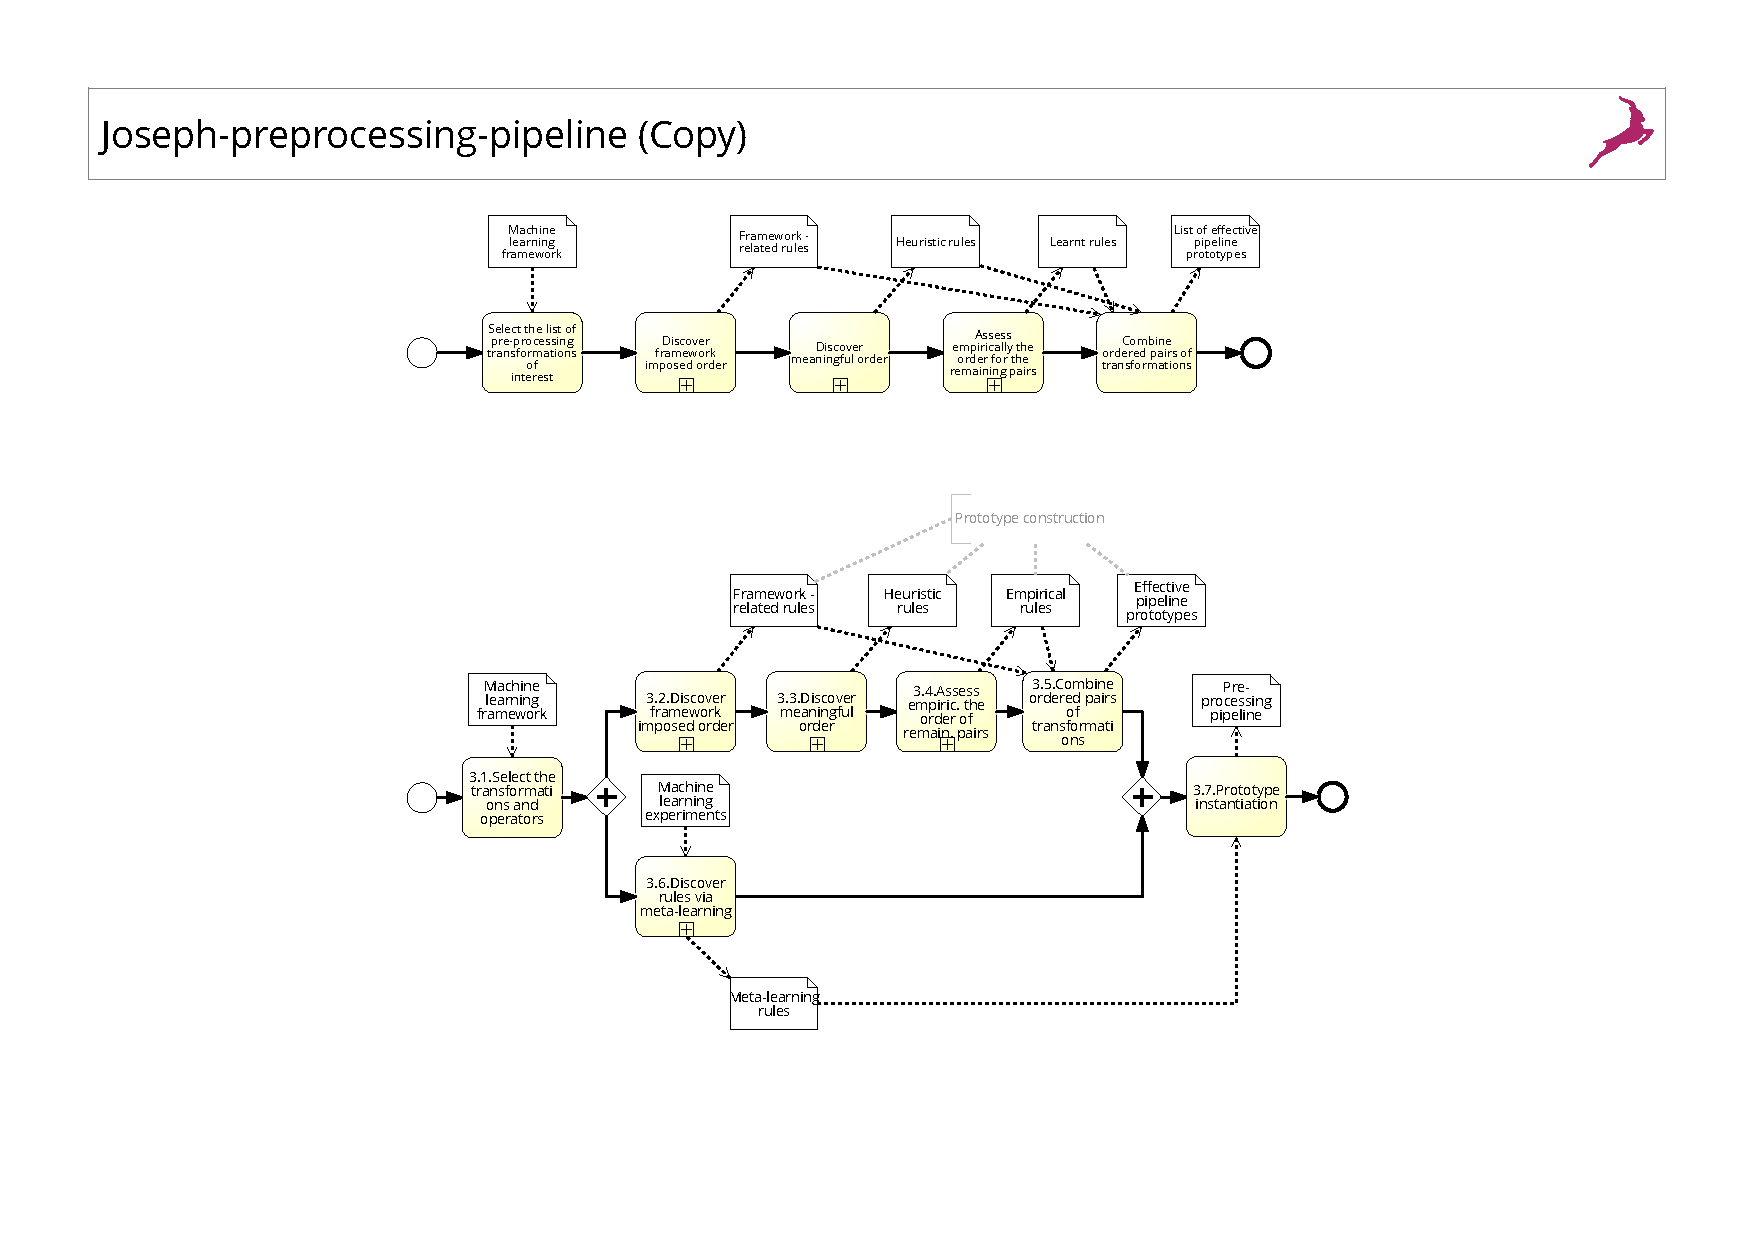
\includegraphics[clip, trim=6.5cm 3.5cm 6.5cm 8cm,width=1.0\textwidth]{chapters/data-centric/supervised/img/bpmn.pdf}
    \caption{A method for generating pre-processing pipelines.}
    \label{fig:methodology}
\end{figure*}

Following the notation from~\cite{Quemy20InfSystems}, we also distinguish between a fixed, ordered sequence of kinds of pre-processing transformations, known as \textit{pipeline prototypes}, and a fixed, ordered sequence of operators (i.e., instantiations of transformations) known as (executable) \textit{pipelines}.
Typically, pipeline prototype construction is a manual and tedious task, where a data scientist exhaustively iterates over a staggeringly large number of possible pipeline orderings, until he/she finds one that works best for the problem at hand. This is a challenging task due to the fact that there are no clear rules and guidelines in terms of which permutation of kinds of transformations would work best (i.e., the final impact of a pipeline is difficult to foresee). To facilitate it, we propose a method, sketched in Figure~\ref{fig:methodology}, that in short breaks the combinatorial problem of finding the best pipeline into studying kinds of transformations in pairs, ultimately, generating effective pipeline prototypes, which are then fed to an optimizer (e.g., we use the SMBO~\cite{HyperOptICML13} variant), to be instantiated and further optimized.
Some of the steps of the method are generic and thus can be applied regardless of the context, and yet others are specific, and depend on the context (i.e., ML framework used or dataset characteristics).


The method consists of two flows running in parallel. The first flow is responsible for the pipeline prototype construction and the second flow allows to generate rules that guide the instantiation of the transformations inside the pipeline prototype. 
The output from the two flows is fed to the final step where the instantiation and optimization happens. The result is an executable pipeline. Notice that what we propose is a generic method, however for the sake of an example, we use the OpenML repository~\cite{OpenML2013}, the Scikit-learn library, and the HyperOpt tool, that internally uses SMBO, to provide a use case.

The proposed method starts with the selection of the ML library and optimization framework to be used. On the one hand, this allows to choose the potential kinds of transformations and their available instantiations, and on the other it allows to generate \textit{framework-related rules}, reflecting the limitations in the concrete implementation of operators. These rules enable the generation of precedence relationships between the kinds of transformations for which they apply.
Next, the flow on top continues with a study over all the possible pairs of kinds of transformations, aiming to find the correct/meaningful order between them using \textit{generic knowledge} about their behaviour. As a result, a set of \textit{heuristic rules} that determines precedences between transformations is generated. 
Afterwards, for the pairs for which an order cannot be clearly devised, an additional empirical study is proposed. This study may rely on a testbed of dataset representatives, and thus it may implicitly correspond to \textit{domain knowledge}. The output of this step is a set of \textit{empirically learned rules} that determines promising precedences of transformations (i.e. an order that would potentially positively impact the final result of the analysis). However, even after this phase, for some pairs of transformations a precedence order may not be found. These are pairs for whom the order is relevant but cannot be decided in advance, thus all their permutations need to be present. Finally, a step of composition follows, where given the overall set of devised rules (i.e., \textit{framework-related}, \textit{heuristic} and \textit{empirically learned}), transformations are composed into a set of valid and potentially effective pipeline prototypes. 

Once the prototype is constructed, the flow running in parallel is proposed to help with its instantiation. It consists of a meta-learning step, where a set of ML experiments (e.g., pre-processing and classification algorithm runs) are used as training data, to predict the initial operator for the transformations inside the pipeline prototype. These rules extract knowledge from past experiments and are complementary to the rules obtained in the first flow. They would be used, for example, to ease the cold start problem in the prototype instantiation phase.

\subsection{Transformations and Operators}

The first task in the process consists of selecting the kinds of transformations and their available operators. 

When combining two different kinds of transformations, it is important to check if, (i) the input and output types of transformations are compatible, (ii) the combination makes sense, and (iii) the combination provides good results for the analysis. As a result, when chaining a pair of transformations, the following precedence relationships arise:

\begin{enumerate}
    \item Compatible/Incompatible pairs. Depending on whether the representation output of the first transformation is accepted as the representation input of the second one (compatible), or not (incompatible) (see Section~\ref{sec:rules-framework}).
    \item Meaningful/Meaningless pairs. Depending on whether the precedence between them makes sense based on generic knowledge (i.e., based on the literature) over the behaviour of transformations (meaningful), or not (meaningless) (see Section~\ref{sec:rules-heuristics}). 
    \item Promising/Unpromising pairs. Depending on whether the precedence between them is expected to provide positive impact on the final result of the analysis (promising), or not (unpromising) (see Section~\ref{sec:rules-learned}). 
\end{enumerate}

Attending to the relationships between its transformations, a prototype can be described as either \textit{compatible}, \textit{well-formed}, or \textit{effective}. A prototype is defined to be \textit{compatible}, if all its precedence relationships are compatible. It is defined as \textit{well-formed}, if all its precedence relationships are both compatible and meaningful. Finally, it is defined as \textit{effective}, if all its precedence relationships are compatible, meaningful, and promising at the same time. In fact, the ultimate goal of our method is to find \textit{effective pipelines}.

\begin{example}
The kinds of transformations selected for the sake of our use case are the following:

\begin{itemize}[noitemsep,topsep=0pt]
\item{Encoding ($E$).} The process of transforming Categorical attributes into Continuous ones.
\item{Normalization ($N$).} The process of normalizing Continuous attributes such that their values fall in the same range.
\item{Discretization ($D$).} The process of transforming Continuous attributes into Categorical ones.
\item{Imputation ($I$).} The process of imputing missing values.
\item{Rebalancing ($R$).} The process of adjusting the class distribution of a dataset (i.e. the ratio between the different classes/categories represented).
\item{Feature Engineering ($F$).} The process of defining the set of relevant attributes (variables, predictors) to be used in model construction.

\end{itemize}

\begin{table}[!t]
\renewcommand{\arraystretch}{0.3}
\footnotesize
\caption{List of transformations applicable to Categorical or Continuous data types.}
\centering
\begin{threeparttable}

\begin{tabular}{@{}p{30mm}lll>{\ttfamily}l@{}}
\toprule
Transf. Kind& Input & Output & Operator & \textnormal{Parameters}
\\	\cmidrule[.1em]{1-5}

Encoding ($E$)  & CA & CO & Ordinal & -  \\ \cmidrule[.05em]{4-5} & & & One Hot & - \\
\cmidrule[.1em]{1-5}

Normalization ($N$) & CO & CO & Standard Scaler & with\_mean:[True,False]\\ \cmidrule[.05em]{4-5} & & & & with\_std:[True,False] \\ \cmidrule[.05em]{4-5}
&  &  & Power Transform & -\\ \cmidrule[.05em]{4-5}
&  &  & MinMax Scaler & -\\ \cmidrule[.05em]{4-5}
&  &  & Robust Scaler & quantile\_range:[(25,75),(10,90),(5,95)]\\ \cmidrule[.05em]{4-5} & & & & with\_centering:[True,False]\\ \cmidrule[.05em]{4-5} & & & & with\_scaling:[True,False] \\
\cmidrule[.1em]{1-5}

Discretization ($D$) & CO & CA & KBins & n\_bins:[3,5,7]\\ \cmidrule[.05em]{4-5} & & & & encode:[`onehot',`onehot-dense',`ord.']\\ \cmidrule[.05em]{4-5} & & & & strategy:[`uniform',`quant.',`kmeans']\\	\cmidrule[.05em]{4-5}
&  &  & Binarization  & threshold: [0, 0.5, 2, 5]\\	\cmidrule[.1em]{1-5}

Imputation ($I$) & CA/CO & CA/CO  & Univariate & strategy:[`most\_freq.','constant'] \\	\cmidrule[.05em]{4-5}
 & &  & Multivariate & initial\_strategy:[`most\_freq',`const.']\\ \cmidrule[.05em]{4-5} & & & & order:[`asc',`dsc',`rom',`arab',`rand'] \\	\cmidrule[.1em]{1-5}

Rebalancing ($R$)* &CA/CO  & CA/CO & Near Miss & n\_neighbors:[1,2,3]\\ \cmidrule[.05em]{4-5}
%&  &  & \textcolor{red}{Condensed KNN} & \textcolor{red}{n\_neighbors:[1,2,3]} \\ \cmidrule[.05em]{4-5}
&  &  & SMOTE & k\_neighbors:[5,6,7]\\	\cmidrule[.1em]{1-5}

Feat. Eng. ($F$) & CA/CO & CA/CO & PCA & n\_components:[1,2,3,4]\\ \cmidrule[.05em]{4-5}
&  &  & Select K Best & k:[1,2,3,4]\\ \cmidrule[.05em]{4-5}
&  &  & PCA + Select K Best  & n\_components:[1,2,3,4]
\\ \cmidrule[.05em]{4-5} & & & & k:[1,2,3,4]\\	\bottomrule%\cmidrule[.1em]{1-5}
\end{tabular}
\begin{tablenotes}
\footnotesize
\item CA - Categorical, CO - Continuous.
\item *All transformations except Rebalancing are taken from scikit-learn.
\end{tablenotes}
\end{threeparttable}
\label{tbl:transformations}
\end{table}

An operator is an actual instantiation/implementation of a kind of transformation. Thus, several operators may implement the same kind of transformation, each having its own set of parameters. For our experiments, we selected the operators and parameters from those available in the Scikit-learn\footnote{\url{https://scikit-learn.org}} library, and they are listed in Table~\ref{tbl:transformations}. \textit{Input} denotes the compatible feature type for a given kind of transformation and can be Continuous (CO) --- when it represents measurements on some continuous scale, or Categorical (CA) --- when it represents information about some categorical or discrete characteristics. Similarly, \textit{Output} denotes the type of the features after a kind of transformation is applied. Finally, \textit{Operator} denotes the physical instantiation for the kind of transformation, and it can be parametrised using its \textit{Parameters}.
\end{example}

\begin{table*}[!t]
    \caption{
        Precedence order between pairs of transformations, represented independently for each phase. 
        }
    \renewcommand{\arraystretch}{0.3}
    \footnotesize
    \begin{center}
    \subfloat[Compatible precedence.]{
    \begin{tabular}{@{}lcccccc}
    \toprule
     & $\boldsymbol{E}$ & $\boldsymbol{N}$ & $\boldsymbol{D}$ & $\boldsymbol{I}$ & $\boldsymbol{R}$ & $\boldsymbol{F}$
    \\	\cmidrule[.1em]{1-7}
    $\boldsymbol{E}$ & \cellcolor{gray!25} & \texttt{1} & \texttt{1} & \texttt{\texttt{0}} & \texttt{1} & \texttt{1} \\	\cmidrule[.1em]{1-7}
    $\boldsymbol{N}$ & \texttt{0} & \cellcolor{gray!25}  & \texttt{0} & \texttt{0} & \texttt{0} & \texttt{0} \\	\cmidrule[.1em]{1-7}
    $\boldsymbol{D}$ & \texttt{0} & \texttt{0} & \cellcolor{gray!25}  & \texttt{0} & \texttt{0} & \texttt{0} \\	\cmidrule[.1em]{1-7}
    $\boldsymbol{I}$ & \texttt{1} & \texttt{0} & \texttt{1} & \cellcolor{gray!25}  & \texttt{1} & \texttt{1} \\	\cmidrule[.1em]{1-7}
    $\boldsymbol{R}$ & \texttt{0} & \texttt{0} & \texttt{0} & \texttt{0} & \cellcolor{gray!25}  & \texttt{0} \\	\cmidrule[.1em]{1-7}
    $\boldsymbol{F}$ & \texttt{0} & \texttt{0} & \texttt{0} & \texttt{0} & \texttt{0} & \cellcolor{gray!25}
    \\	\bottomrule
    \end{tabular}}
    \qquad% --- set horizontal distance between tables here
    \subfloat[Meaningful precedence.]{%
    \begin{tabular}{@{}lcccccc}
    \toprule
    & $\boldsymbol{E}$ & $\boldsymbol{N}$ & $\boldsymbol{D}$ & $\boldsymbol{I}$ & $\boldsymbol{R}$ & $\boldsymbol{F}$
    \\	\cmidrule[.1em]{1-7}
    $\boldsymbol{E}$ & \cellcolor{gray!25} & \texttt{0} & \texttt{0} & \texttt{0} & \texttt{0} & \texttt{0} \\	\cmidrule[.1em]{1-7}
    $\boldsymbol{N}$ & \texttt{0} & \cellcolor{gray!25}  & \texttt{X} & \texttt{0} & \texttt{1} & \texttt{0} \\	\cmidrule[.1em]{1-7}
    $\boldsymbol{D}$ & \texttt{0} & \texttt{X} & \cellcolor{gray!25}  & \texttt{0} & \texttt{0} & \texttt{0} \\	\cmidrule[.1em]{1-7}
    $\boldsymbol{I}$ & \texttt{1} & \texttt{1} & \texttt{1} & \cellcolor{gray!25}  & \texttt{1} & \texttt{1} \\	\cmidrule[.1em]{1-7}
    $\boldsymbol{R}$ & \texttt{0} & \texttt{0} & \texttt{0} & \texttt{0} & \cellcolor{gray!25}  & \texttt{0} \\	\cmidrule[.1em]{1-7}
    $\boldsymbol{F}$ & \texttt{0} & \texttt{0} & \texttt{0} & \texttt{0} & \texttt{0} & \cellcolor{gray!25}
    \\	\bottomrule
    \end{tabular}}
    \qquad% --- set horizontal distance between tables here
    \subfloat[Promising precedence.]{%
    \begin{tabular}{@{}lcccccc}
    \toprule
    & $\boldsymbol{E}$ & $\boldsymbol{N}$ & $\boldsymbol{D}$ & $\boldsymbol{I}$ & $\boldsymbol{R}$ & $\boldsymbol{F}$
    \\	\cmidrule[.1em]{1-7}
    $\boldsymbol{E}$ & \cellcolor{gray!25} & \texttt{0} & \texttt{0} & \texttt{0} & \texttt{0} & \texttt{0} \\	\cmidrule[.1em]{1-7}
    $\boldsymbol{N}$ & \texttt{0} & \cellcolor{gray!25} & \texttt{0} & \texttt{0} & \texttt{0} & \texttt{1} \\	\cmidrule[.1em]{1-7}
    $\boldsymbol{D}$ & \texttt{0} & \texttt{0} & \cellcolor{gray!25} & \texttt{0} & \texttt{0} & \texttt{1} \\	\cmidrule[.1em]{1-7}
    $\boldsymbol{I}$ & \texttt{0} & \texttt{0} & \texttt{0} & \cellcolor{gray!25} & \texttt{0} & \texttt{0} \\	\cmidrule[.1em]{1-7}
    $\boldsymbol{R}$ & \texttt{0} & \texttt{0} & \texttt{0} & \texttt{0} & \cellcolor{gray!25} & \texttt{0} \\	\cmidrule[.1em]{1-7}
    $\boldsymbol{F}$ & \texttt{0} & \texttt{0} & \texttt{0} & \texttt{0} & \texttt{0} & \cellcolor{gray!25} 
    \\	\bottomrule
    \end{tabular}}
    \end{center}
    \begin{tablenotes}
    \centering
    \scriptsize
    \item$\boldsymbol{E}$ - Encoding; $\boldsymbol{N}$ - Normalization; $\boldsymbol{D}$ - Discretization; $\boldsymbol{I}$ - Imputation; $\boldsymbol{R}$ - Rebalancing; $\boldsymbol{F}$ - Feature Engineering. \item \texttt{1} - a precedence edge exists between the row and the column, \texttt{0} - a precedence edge does not exist between the row 
    \item and the column, \texttt{X} - the combination is meaningless.
    \end{tablenotes}
    \label{tbl:rules}
    \end{table*}

\subsection{Framework-related rules}
\label{sec:rules-framework}
Once the implementation framework is selected, one needs to study it and see if there exist constraints that limit the interaction between transformations. For instance, applying a transformation may actually invalidate the application of another transformation, because the compatibility of transformations is dependent on the selected ML framework.

\begin{example}
We studied the transformations implemented in Scikit-learn and detected a set of implicit rules that are shown through an adjacency matrix, corresponding to a precedence graph, in Table~\ref{tbl:rules}a.
Each cell $a_{ij}$ denotes a precedence relationship between the row $i$ and column $j$. Hence, \texttt{1} means that an edge exists between the transformation in the row and the transformation in the column, whereas \texttt{0} means that such an edge does not exist, hence a precedence order is not established for that pair. 
For example, most Scikit-learn transformations cannot be applied in the presence of missing values. This is why in every pair of transformations where Imputation is involved, except the one with Normalization\footnote{Normalization transformations are the only ones that Scikit-learn can apply on datasets with missing values.}, Imputation goes first.
Furthermore, Scikit-learn transformations are applied only to all compatible attributes of a given dataset. Generally, Categorical attributes are physically represented as strings and Continuous attributes as numbers. However, a transformation that is meant to be applied, say to Continuous attributes, cannot be applied over a dataset that contains both Continuous and Categorical attributes (i.e., a dataset containing both numbers and strings); Scikit-learn cannot deal with arrays of mixed types. In that case, all the Categorical attributes need to be encoded into numeric representations, even if they represent a categorical value. That is, a value can be a number but represent a category. 
This is what happens when Normalization and Discretization are meant to be applied to a dataset containing mixed types of attributes. In order for them to be applied to datasets of mixed types, an Encoding transformation needs to be applied first. A similar constraint is imposed when considering Rebalancing and Feature Engineering, since these transformations do not accept inputs containing strings (i.e., representing a Categorical type). 
For the rest of the pairs of transformations there are no constraints imposed by the framework, thus any order of such transformations is permitted, reflected by a \texttt{0} in Table~\ref{tbl:rules}a.
The graph obtained in this case exclusively corresponds to the limitations of Scikit-learn (as a matter of fact, if another framework were to be chosen, it may have looked differently).
\end{example}

\begin{algorithm*}[!h]
	\caption{Find a promising pipeline prototype for transformations $T_1$ and $T_2$}
	\label{alg:learned-rules}
	\begin{algorithmic}[1]
		\Require $d$, $a$ \Comment{dataset, classification algorithm}
		\Require \indent$T_1\rightarrow T_2$, $T_2 \rightarrow T_1$ \Comment{precedence orders of a pair of transformations}
		\State $acc_{baseline} = Acc(d,a)$; \Comment{get baseline performance of algorithm on d}
		\State $[pipeline_{T_1\rightarrow T_2},acc_{T_1\rightarrow T_2}] = SMBO(T_1\rightarrow T_2,d, a)$
		\Comment{get pipeline and accuracy for $T_1\rightarrow T_2$}
		\State $[pipeline_{T_2\rightarrow T_1},acc_{T_2\rightarrow T_1}] = SMBO(T_2\rightarrow T_1,d, a)$
		\Comment{get pipeline and accuracy for $T_2\rightarrow T_1$}
		\If{\textit{IsValid}($acc_{T_1\rightarrow T_2},acc_{T_2\rightarrow T_1},acc_{baseline}$)}
        \Comment{see Table~\ref{tbl:validation-rules} for the rules applied}
        \State \Return \textit{Winner}$([pipeline_{T_1\rightarrow T_2},acc_{T_1\rightarrow T_2}],[pipeline_{T_2\rightarrow T_1},acc_{T_2\rightarrow T_1}])$ 
        \Comment{see column \textit{Winner prototype} in Table~\ref{tbl:validation-rules}}
		\Else
		\State \Return $\varnothing$
		\EndIf
	\end{algorithmic}
\end{algorithm*}

\subsection{Heuristic rules}
\label{sec:rules-heuristics}
In the previous section, we proposed to derive a precedence based on the constraints of the framework. Now, we want to study the precedence independently of the framework, and find \textit{meaningful pairs}. That is, for every given pair, we want to find the relative order, based on generic, domain-independent knowledge (i.e., literature) about transformations and their applicability. To this end, some of the constraints imposed by the framework may be contradicted here, but this is resolved in the last step of the proposed method, when we take the union of the rules and hence construct the final pipeline prototypes (see Section~\ref{sec:composition}). Briefly, in a combination where Imputation is involved, it is advised to apply Imputation first. Next, an Encoding transformation makes sense to be combined in any order with the rest of transformations, except Imputation. 
Combining Discretization with Normalization does not make sense, due to the fact that after the Discretization step, Continuous attributes are transformed into Categorical ones, and hence Normalization cannot be applied. Similarly, applying Normalization first, changes the scale of the values and hence impacts the Discretization step. Finally, a meaningful precedence can be derived when combining Normalization with Rebalancing. In this case, Normalization should be applied first, since otherwise Rebalancing would impact the scale of the values to be normalized.

\begin{example}
For our use case, Table~\ref{tbl:rules}b shows the heuristic rules obtained considering domain-independent knowledge about transformations~\cite{BookExploratoryDM03Dasu}. In comparison with the results from Table~\ref{tbl:rules}a, observe that the constraints on the Imputation transformation still hold, that is, it is correct to apply Imputation first when combining it with another transformation. This time even when combining it with Normalization --- note the difference with Table~\ref{tbl:rules}a. The constraints of Encoding are however not present in Table~\ref{tbl:rules}a, hence not considering the framework, Discretization combined with Encoding is a meaningful combination --- when a mixed type dataset is considered, but incompatible from the point of view of Scikit-learn.
\end{example}

\subsection{Empirically learned rules}
\label{sec:rules-learned}

The two previously proposed steps (i.e., \textit{framework-related} and \textit{heuristic rules}), do not guarantee that for each pair of transformations we will obtain a precedence order. Therefore, for the cases where they are not sufficient to determine the precedence, a third viewpoint can be considered. That of learning a promising order by empirically studying the impact of the combinations on the final result of the analysis, using different classification problems in the training. For every selected pair of transformations, for a given classification algorithm, we propose to check which order of the pair improves most the performance (e.g., predictive accuracy) of the algorithm over a set of datasets (preferably from different domains). Like this, for each dataset we can get a precedence order that gives better results (i.e., promising precedence) in terms of predictive accuracy (other metrics can be used as well). 

\paragraph{Algorithm}
\label{sec:rules-learned:algorithm}

\begin{table*}[t]
\footnotesize
\centering
\begin{threeparttable}
\caption{
    Validation rules.
    }
\begin{tabular}{@{}lllllc@{}}
\toprule
Nr. & Pipeline 1 & Pipeline 2 & Valid result & Valid score & Winner prototype\\\toprule
         1. &$\varnothing \rightarrow \varnothing$ & $\varnothing \rightarrow \varnothing$ & Draw          & $acc_{baseline}$ &  Baseline \\ \hline
        2. &$\varnothing \rightarrow \varnothing$ & $con\!f_{T_2} \rightarrow \varnothing$ & Draw          & $acc_{baseline}$ & Baseline \\ \hline
        3. &$\varnothing \rightarrow \varnothing$ & $\varnothing \rightarrow con\!f_{T_1}$ & Draw          & $acc_{baseline}$ & Baseline \\ \hline
        \multirow{2}{*}{4.} &\multirow{2}{*}{$\varnothing \rightarrow \varnothing$} & \multirow{2}{*}{$con\!f_{T_2} \rightarrow con\!f_{T_1}$} & Draw & $acc_{baseline}$ & Baseline \\
        & & & $con\!f_{T_2} \rightarrow con\!f_{T_1}$ & $acc_{T_2 \rightarrow  T_1}$ & $T_2 \rightarrow T_1$\\ \hline
        5. & $\varnothing \rightarrow con\!f_{T_2}$ & $\varnothing \rightarrow \varnothing$ & Draw          & $acc_{baseline}$ & Baseline \\ \hline
        \multirow{3}{*}{6.} & \multirow{3}{*}{$\varnothing \rightarrow con\!f_{T_2}$} & \multirow{3}{*}{$con\!f_{T_2} \rightarrow \varnothing$} & Draw &  \multirow{3}{*}{$acc_{T_2}$}  & $T_2$ \\
        & & & $\varnothing \rightarrow con\!f_{T_2}$ & & $T_2$ \\
        & & & $con\!f_{T_2} \rightarrow \varnothing$ & & $T_2$ \\ \hline
        7. &$\varnothing \rightarrow con\!f_{T_2}$ & $\varnothing \rightarrow con\!f_{T_1}$ & Draw & $acc_{T_2}$ or $acc_{T_1}$ & $T_{1}\,or\, T_2$ \\ \hline
        \multirow{2}{*}{8.} & \multirow{2}{*}{$\varnothing \rightarrow con\!f_{T_2}$} & \multirow{2}{*}{$con\!f_{T_2} \rightarrow con\!f_{T_1}$} & Draw & $acc_{T_2}$ & $T_2$\\
        & & & $con\!f_{T_2} \rightarrow con\!f_{T_1}$ & $acc_{T_2 \rightarrow  T_1}$ & $T_2 \rightarrow T_1$ \\ \hline
        9. & $con\!f_{T_1} \rightarrow \varnothing$ & $\varnothing \rightarrow \varnothing$ & Draw & $acc_{baseline}$ & Baseline \\ \hline
        10. & $con\!f_{T_1} \rightarrow \varnothing$ & $con\!f_{T_2} \rightarrow \varnothing$ & Draw & $acc_{T_1}$ or $acc_{T_2}$ & $T_{1}\,or\, T_2$ \\ \hline
        \multirow{3}{*}{11.} & \multirow{3}{*}{$con\!f_{T_1} \rightarrow \varnothing$} & \multirow{3}{*}{$\varnothing \rightarrow con\!f_{T_1}$} & Draw & \multirow{3}{*}{$acc_{T_1}$} & $T_1$\\
        & & & $con\!f_{T_1} \rightarrow \varnothing$ & & $T_1$\\
        & & & $\varnothing \rightarrow con\!f_{T_1}$ & & $T_1$\\ \hline
        \multirow{2}{*}{12.} & \multirow{2}{*}{$con\!f_{T_1} \rightarrow \varnothing$} & \multirow{2}{*}{$con\!f_{T_2} \rightarrow con\!f_{T_1}$} & Draw & $acc_{T_1}$  & $T_1$\\
        & & & $con\!f_{T_2} \rightarrow con\!f_{T_1}$ & $acc_{T_2 \rightarrow  T_1}$ & $T_2 \rightarrow T_1$ \\ \hline
        \multirow{2}{*}{13.} & \multirow{2}{*}{$con\!f_{T_1} \rightarrow con\!f_{T_2}$} & \multirow{2}{*}{$\varnothing \rightarrow \varnothing$} & Draw & $acc_{baseline}$  & Baseline\\
        & & & $con\!f_{T_1} \rightarrow con\!f_{T_2}$ & $acc_{T_1 \rightarrow  T_2}$ & $T_1 \rightarrow T_2$ \\ \hline
        \multirow{2}{*}{14.} & \multirow{2}{*}{$con\!f_{T_1} \rightarrow con\!f_{T_2}$} & \multirow{2}{*}{$con\!f_{T_2} \rightarrow \varnothing$} & Draw & $acc_{T_2}$ & $T_2$\\
        & & & $con\!f_{T_1} \rightarrow con\!f_{T_2}$ & $acc_{T_1 \rightarrow  T_2}$  & $T_1 \rightarrow T_2$ \\ \hline
        \multirow{2}{*}{15.} & \multirow{2}{*}{$con\!f_{T_1} \rightarrow con\!f_{T_2}$} & \multirow{2}{*}{$\varnothing \rightarrow con\!f_{T_1}$} & Draw & $acc_{T_1}$ & $T_1$\\
        & & & $con\!f_{T_1} \rightarrow con\!f_{T_1}$ & $acc_{T_1 \rightarrow  T_2}$ & $T_1 \rightarrow T_2$\\ \hline
        \multirow{3}{*}{16.} & \multirow{3}{*}{$con\!f_{T_1} \rightarrow con\!f_{T_2}$} & \multirow{3}{*}{$con\!f_{T_2} \rightarrow con\!f_{T_1}$} & Draw & $acc_{T_1}$ or $acc_{T_2}$ & $T_{1}\,or\, T_2$ \\
        & & & $con\!f_{T_1} \rightarrow con\!f_{T_2}$ & $acc_{T_1 \rightarrow  T_2}$ & $T_1 \rightarrow T_2$\\
        & & & $con\!f_{T_2} \rightarrow con\!f_{T_1}$ & $acc_{T_2 \rightarrow  T_1}$ & $T_2 \rightarrow T_1$\\ \bottomrule
\end{tabular}
\begin{tablenotes}
\footnotesize
\item $\varnothing$ - SMBO finds a better result without instantiating a transformation (or both) in the pair.
\item $con\!f_T$ - The configuration (i.e., operator and its parameters) found for $T$ by SMBO.
\item $acc_T$ - The accuracy of the ML algorithm over the data transformed with a pipeline $T$.
\end{tablenotes}
    \label{tbl:validation-rules}
\end{threeparttable}
\end{table*}

\begin{figure*}[!b]
	\centering
	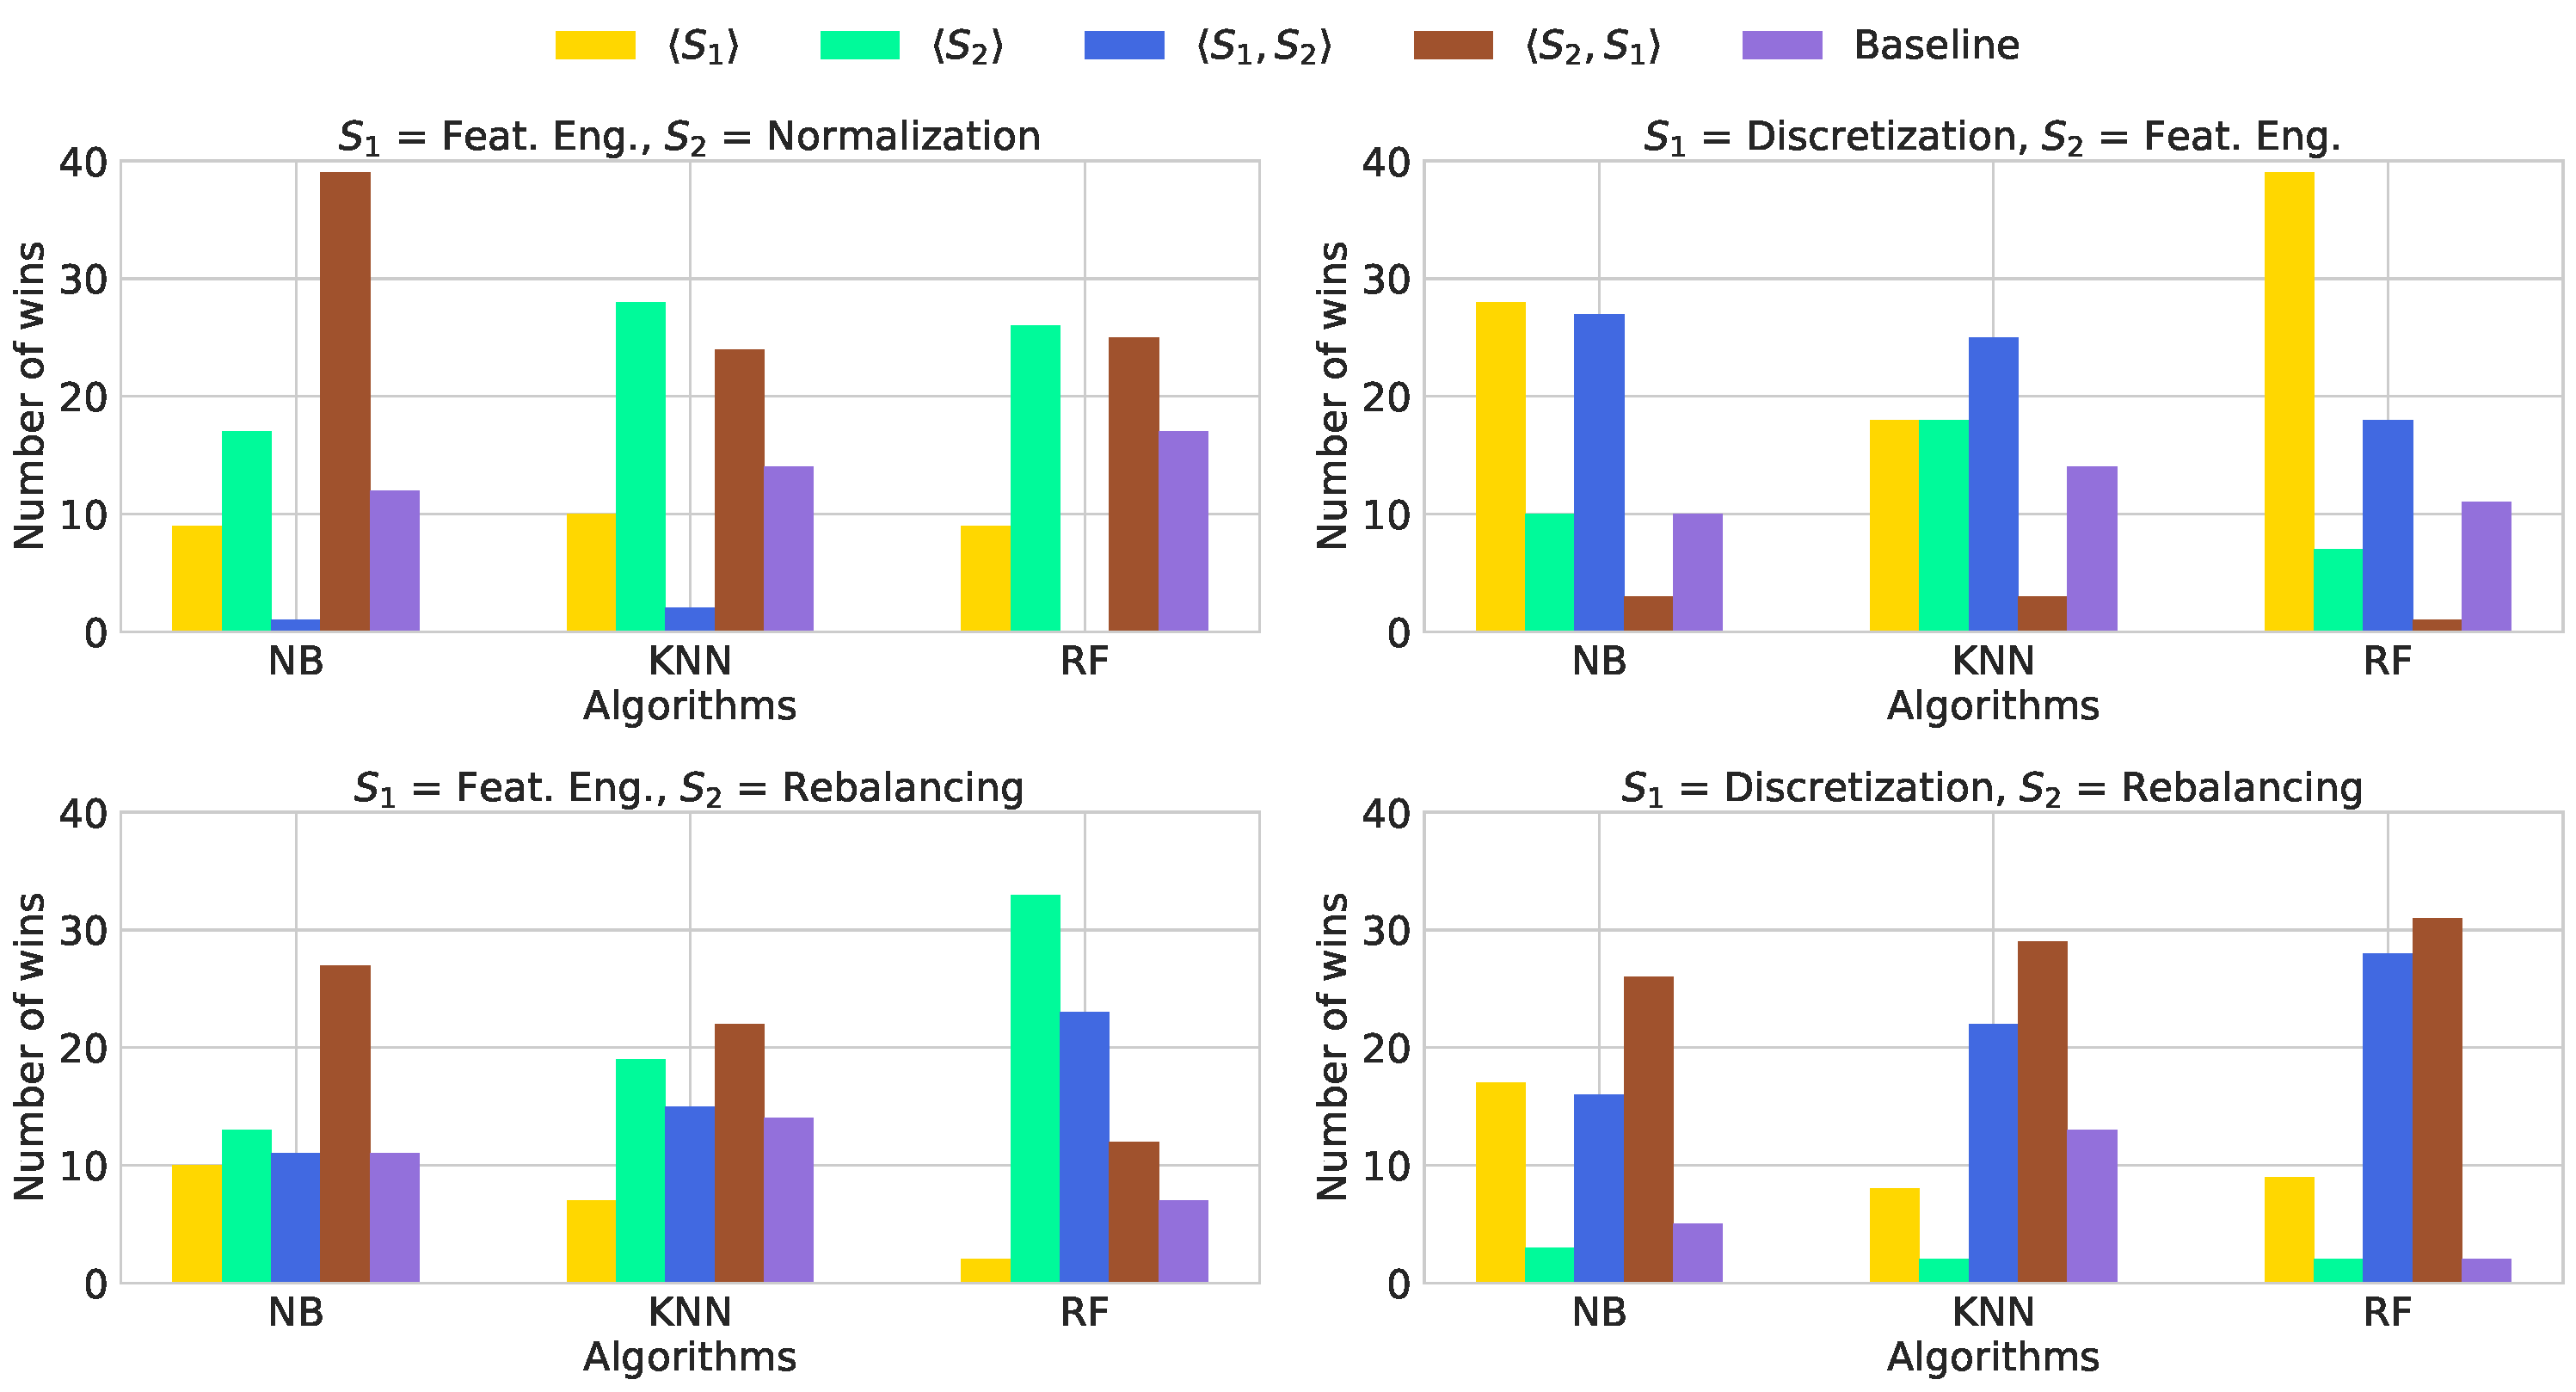
\includegraphics[width=1.0\textwidth]{chapters/data-centric/supervised/img/experiments_results.pdf}
	\caption{Number of datasets for which a given pipeline prototype is declared the winner.}
	\label{fig:learned-rules-results}
\end{figure*}

To find a promising precedence order between a given pair of transformations, we propose Algorithm~\ref{alg:learned-rules}. 
To compute the impact of transformations, we first get the accuracy of the ML algorithm over the original non-transformed dataset (see line 1). %, which is used later for calculating the change in accuracy. 
Afterwards, for each precedence order between the pairs of transformations, we find both their optimized executable pipelines (i.e., using SMBO), and the accuracies of the ML algorithm (with default parametrisation) over the datasets transformed using the respective pipelines (see lines 2-3). Based on the comparison between the respective optimized pipelines, we get the winner in line 5. However, beforehand, in line 4, we perform a validity check. This is because when optimizing a pre-processing pipeline, SMBO may not instantiate a transformation with an operator at all (i.e., represented with a $\varnothing$ symbol).
Hence, given a pair of transformations, where one or both of them may not be instantiated, SMBO may generate 16 possible scenarios. They are listed in Table~\ref{tbl:validation-rules}, and make up the validation rules for Algorithm~\ref{alg:learned-rules} (see line 4). 

Briefly, if among the optimized pairs of transformations (same transformations but in reverse order) obtained from SMBO, one or both of them contain a $\varnothing$ operator, their results are considered valid, only if they have equal scores (i.e., a draw). This is because, if one has a higher score, it means that during the optimization phase it was more advantageous than the other, since it could find a configuration that should have been found by both of the pairs, given enough budget. In our SMBO runs, such invalid results account for less than 10\% and in those cases datasets are discarded from the study (see line 7). 

In particular, in Table~\ref{tbl:validation-rules}, the first two columns denote the pipeline instantiations for the respective pairs of transformations (i.e., $T_1\rightarrow T_2$ and $T_2\rightarrow T_1$). Next, \textit{Valid result} denotes the expected result when comparing the results of the pipelines in the same row. For instance, in the first row, if both transformations in the pipelines are not instantiated during the optimization, a valid result is a draw, and a \textit{Valid score} for the respective result is the baseline accuracy, and the \textit{Winner prototype} is the prototype that is in accordance with the expected result, which in this case is the Baseline (i.e., prototype consisting of only the ML algorithm, where no transformations are applied).

For the sake of another example, let us check row 2 in Table~\ref{tbl:validation-rules}. Running SMBO, the best result for the first pair is the pipeline $\varnothing \rightarrow \varnothing$, and for the second pair, the pipeline $T_2 \rightarrow \varnothing$. In this case, the comparison between the results of these pipelines should be equal (i.e., draw), and the score should be that of the baseline. Otherwise, if say, the score of the second pipeline was higher, it would mean that for the first pair, SMBO was not given enough time to find the pipeline with higher score (i.e., $T_2\rightarrow \varnothing$).
The same logic applies also for the other rows where a $\varnothing$ operator is involved.

\color{black}

\begin{example}
For the sake of this work, we considered three classification algorithms (i.e., \textit{NB}, \textit{RF},  \textit{KNN}) and 80 datasets from the OpenML repository. The datasets, were compiled from three OpenML benchmarks, namely, the OpenMLCC18 benchmark\footnote{\url{https://www.openml.org/s/99/data}}, the AutoML benchmark\footnote{\url{https://www.openml.org/s/271/data}}, and the Classification algorithms benchmark\footnote{\url{https://www.openml.org/s/1/data}}. For the final set, we filtered out datasets with more than 10\% of missing values --- not to include bias due to the heavy pre-processing we need to perform on top of them, and we filtered out the datasets with more than 5 million instances --- because of the computation time required to process them. As a result we obtained 60 datasets from the first benchmark, 17 from the second, and 3 more from the third to reach a total of 80 datasets. 

Given the proposed algorithm (i.e. Algorithm~\ref{alg:learned-rules}), we could try to learn the precedence of every pair of transformations, but would just be a waste of resources, because we can see in Table~\ref{tbl:rules}a and~\ref{tbl:rules}b, that some precedences are already decided for one reason or another. Hence, only pairs of transformations with a \texttt{0} for both directions (in both Table~\ref{tbl:rules}a and~\ref{tbl:rules}b) need to be studied further. That is, they make sense to be combined together, but a precedence order could not be determined through \textit{framework-related} or \textit{heuristic rules}. % for them. 
Thus, for instance, pairs involving Encoding are not considered in this phase, since for them an order is already imposed by the framework (see Table~\ref{tbl:rules}a).
To this end, the pairs of transformations we consider for the third precedence graph include only $\{F,N\}$, $\{F,D\}$, $\{F,R\}$, and $\{R,D\}$.

\begin{table}[t]
	\centering
	\footnotesize
	\begin{threeparttable}
		\caption{
			Binomial test for determining the order between pairs of transformations. 
		}
		\label{tbl:significance-test}
		\begin{tabular}{@{}cccccc@{}}
			\toprule
			%$T_1$ & $T_2$ & $T_1 \rightarrow T_2$ & $T_2 \rightarrow T_1$ & alpha & \begin{tabular}[c]{@{}c@{}}p-value\\ $H_0:\pi = \pi_0=0.8$\end{tabular} \\ \midrule
			$T_1$ & $T_2$ & $T_1 \rightarrow T_2$ & $T_2 \rightarrow T_1$ & alpha & p-value\\ \midrule
			$F$ & $N$ & 3 & 88 & 0.05 &  \textbf{0} \\
			$D$ & $F$ & 70 & 7 & 0.05 &  \textbf{0}  \\
			$F$ & $R$ & 49 & 61 & 0.05 & 8.53e-01 \\
			$D$ & $R$ & 66 & 86 & 0.05 & 9.38e-01 \\ \bottomrule
		\end{tabular}
		\begin{tablenotes}
		\centering
		\scriptsize
		\item$N$ - Normalization; $D$ - Discretization; $R$ - Rebalancing; $F$ - Feature Engineering. 
		\end{tablenotes}
	\end{threeparttable}
\end{table}
Applying Algorithm~\ref{alg:learned-rules}, we obtain a pro\-mising order for each pair of transformations considered. %(i.e., $\{F,N\}$, $\{F,D\}$, $\{F,R\}$, $\{R,D\}$). 
Since SMBO is a randomized algorithm we experimented with (i) running it several times splitting the budget, and (ii) running it only once with the entire budget. For the experiments considered, no significant differences where observed, therefore we opted for running it once with the entire budget (i.e., 200 seconds per run), which allows for more configurations to be visited in a single run. Aggregating all the results, Figure~\ref{fig:learned-rules-results} shows the number of datasets, for which a given prototype (see Table~\ref{tbl:validation-rules}, column \textit{Winner prototype} for the list of labels) is selected as the winner. For instance, for the pair $\{F,N\}$ (i.e., Feature Engineering, Normalization), the prototype winning in more datasets for \textit{KNN} and \textit{NB} is $N\rightarrow F$. This means that in general, better results are obtained if Normalization is applied before Feature Engineering. 

Next, only $N$ appears as first for \textit{RF} and second best for \textit{KNN} and \textit{NB}, which means that for many datasets, considering different algorithms, it results better to apply only Normalization without combining it with Feature Engineering. The third position is for $\varnothing\rightarrow \varnothing$, which means that for some datasets it is better not to apply any of the transformations (in any combination). The remaining prototypes winning in some datasets are $F$ (only Feature Engineering), and $F \rightarrow N$ (Feature Engineering preceding Normalization).  Finally, for three datasets, that are omitted from the figure, there were no winning pipelines (i.e., pipelines resulted in a draw).

Since our goal is to find the best order for a pair of transformations, we focus on the performances of the pipelines where both of the transformations are instantiated (i.e., $T_1\rightarrow T_2$ versus $T_2\rightarrow T_1$). To do this, we check whether the difference between the number of datasets where they each appear to win are statistically significant by running a binomial test assuming a theoretical probability of 0.5. The results are shown in Table~\ref{tbl:significance-test}.
In summary, the results from Table~\ref{tbl:significance-test} indicate that, with 95\% confidence we can assume that for the pair $\{F,N\}$, $N\rightarrow F$ performs better than $F\rightarrow N$, hence Normalization should precede Feature Engineering. On the other hand, for $\{D,F\}$, $D\rightarrow F$ performs better than $F\rightarrow D$, hence Discretization should precede Feature Engineering. Finally, for the remaining transformations, $\{F,R\}$ and $\{R,D\}$, a precedence order can not be pre-assumed since the results obtained are not significant. 
Using these results, we create the \textit{Promising precedence} adjacency matrix shown in Table~\ref{tbl:rules}c, where as one can observe, precedence edges are introduced for $\{N,F\}$ and $\{D,F\}$, but no edges exist neither for $\{F,R\}$, nor for $\{R,D\}$. 
\end{example}

\paragraph{Cross-validation}
\label{sec:learned-rules-validation}
After running Algorithm~\ref{alg:learned-rules} to empirically find a winner between two pairs of transformations, we may obtain a different distribution of the number of wins for the pairs, depending on the datasets considered. To show that the results obtained with the initial set of datasets are generalizable, we propose to perform an additional cross-validated experiment, where the set of datasets considered can be randomly split into many folds. Then, for each fold, the results can be compared to the rest, with the aim of checking whether the distributions are similar. This check can be done via a significance test (e.g., chi-square). To this end, if the distributions between the folds are similar, it means that the obtained results are independent of the datasets considered, since no matter the combination of the datasets, the results are the same and thus generalizable.


\color{black}

\begin{example}
In our use case, to show that the results do not depend on the datasests selected, we re-run the experiments (i.e., 10-times each), but this time splitting the datasets into 4-folds. The goal was to check if the results of the precedence orders from the different folds (i.e., for each experiment considering a randomly different set of datasets) are similar between them (i.e., follow the same distributions).
To confirm this hypothesis, we perform a chi-square test between the results (precedence orders) obtained in a single fold in comparison to the three remaining folds, hence comparing 25\% of the datasets to the rest. 
In particular, to confirm the hypothesis, we need to find results that accept the null hypothesis of the chi-square test which states that "there is no significant difference between the distributions". To do that, sticking to the 95\% confidence interval, we need to look for p-values greater than 0.05. That is, the higher the p-values, the more we accept the null hypothesis, the more similar the distributions. Looking at the p-values we found out that they were all much higher than 0.05. Specifically, the scores of the chi-square tests of the folds (one fold compared to the rest) are averaged and, after having repeated this procedure 10 times, instead of using a table we depict the 10 averaged p-values using box-plots in Figure~\ref{fig:10-times-4-cv}.
We conclude that, for both of the rules (i.e.,  $F\rightarrow N$ and $F\rightarrow D$), the significance test indicates a compliance between the new results (Figure~\ref{fig:10-times-4-cv}) and those illustrated above (Table~\ref{tbl:significance-test}).



\begin{figure*}[!t]
	\centering
	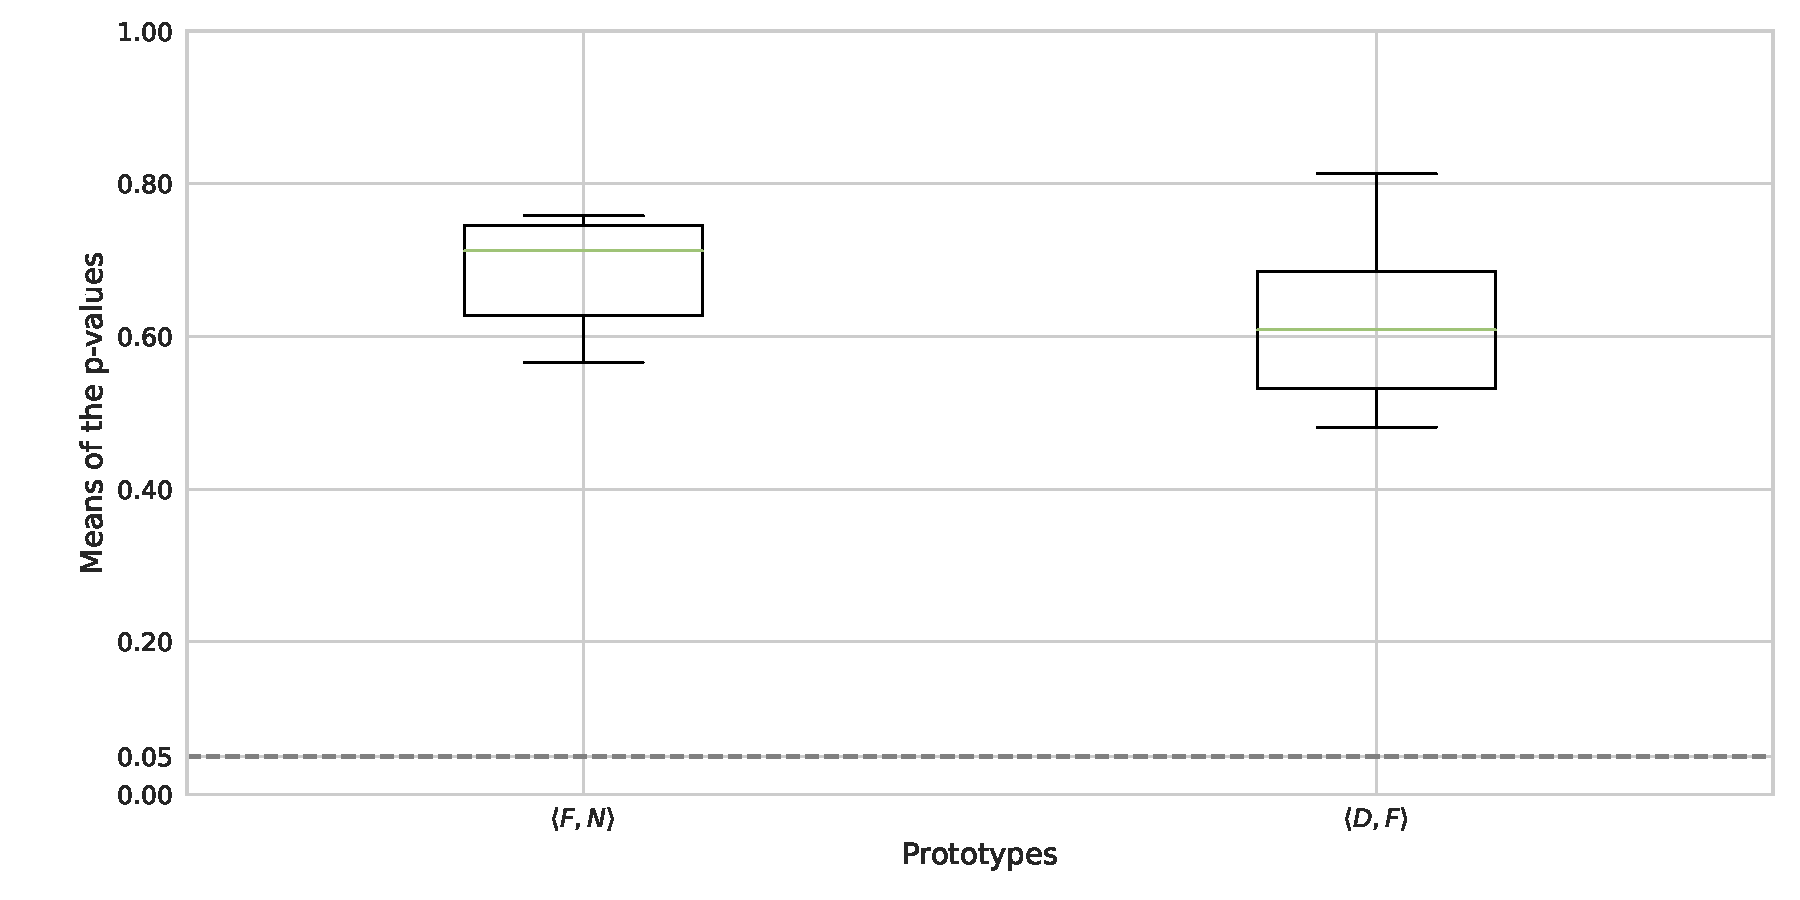
\includegraphics[width=0.9\textwidth]{chapters/data-centric/supervised/img/10_times_4_folds_cv.pdf}
	\caption{The distribution of the p-values obtained after repeating the chi-square test for 10 times, for the 10 times 4-fold cross-validation.}
	\label{fig:10-times-4-cv}
\end{figure*}

\begin{table}[b]
	\caption{
		Union of rules from Table~\ref{tbl:rules}. $\boldsymbol{E}$ - Encoding; $\boldsymbol{N}$ - Normalization; $\boldsymbol{D}$ - Discretization; $\boldsymbol{I}$ - Imputation; $\boldsymbol{R}$ - Rebalancing; $\boldsymbol{F}$ - Feature Engineering \texttt{1} - an edge exists, \texttt{0} - edge does not exist, \texttt{X} - the combination is meaningless.
	}
	\renewcommand{\arraystretch}{0.3}
	\footnotesize
	\centering
	\label{tbl:rules-union}
	\begin{threeparttable}
		\begin{tabular}{@{}lcccccc}
			\toprule
			& $\boldsymbol{E}$ & $\boldsymbol{N}$ & $\boldsymbol{D}$ & $\boldsymbol{I}$ & $\boldsymbol{R}$ & $\boldsymbol{F}$
			\\	\cmidrule[.1em]{1-7}
			$\boldsymbol{E}$ & \cellcolor{gray!25} & \texttt{1} & \texttt{1} & \texttt{0} & \texttt{1} & \texttt{1} \\	\cmidrule[.1em]{1-7}
			$\boldsymbol{N}$ & \texttt{0} & \cellcolor{gray!25}  & \texttt{X} & \texttt{0} & \texttt{1} & \texttt{1} \\	\cmidrule[.1em]{1-7}
			$\boldsymbol{D}$ & \texttt{0} & \texttt{X} & \cellcolor{gray!25} & \texttt{0} & \texttt{0} & \texttt{1} \\	\cmidrule[.1em]{1-7}
			$\boldsymbol{I}$ & \texttt{1} & \texttt{1} & \texttt{1} & \cellcolor{gray!25}  & \texttt{1} & \texttt{1} \\	\cmidrule[.1em]{1-7}
			$\boldsymbol{R}$ & \texttt{0} & \texttt{0} & \texttt{0} & \texttt{0} & \cellcolor{gray!25}  & \texttt{0} \\	\cmidrule[.1em]{1-7}
			$\boldsymbol{F}$ & \texttt{0} & \texttt{0} & \texttt{0} & \texttt{0} & \texttt{0} & \cellcolor{gray!25} \\	\cmidrule[.1em]{1-7}
		\end{tabular}
	\end{threeparttable}
\end{table}

\begin{figure}
\begin{floatrow}
\ffigbox{
    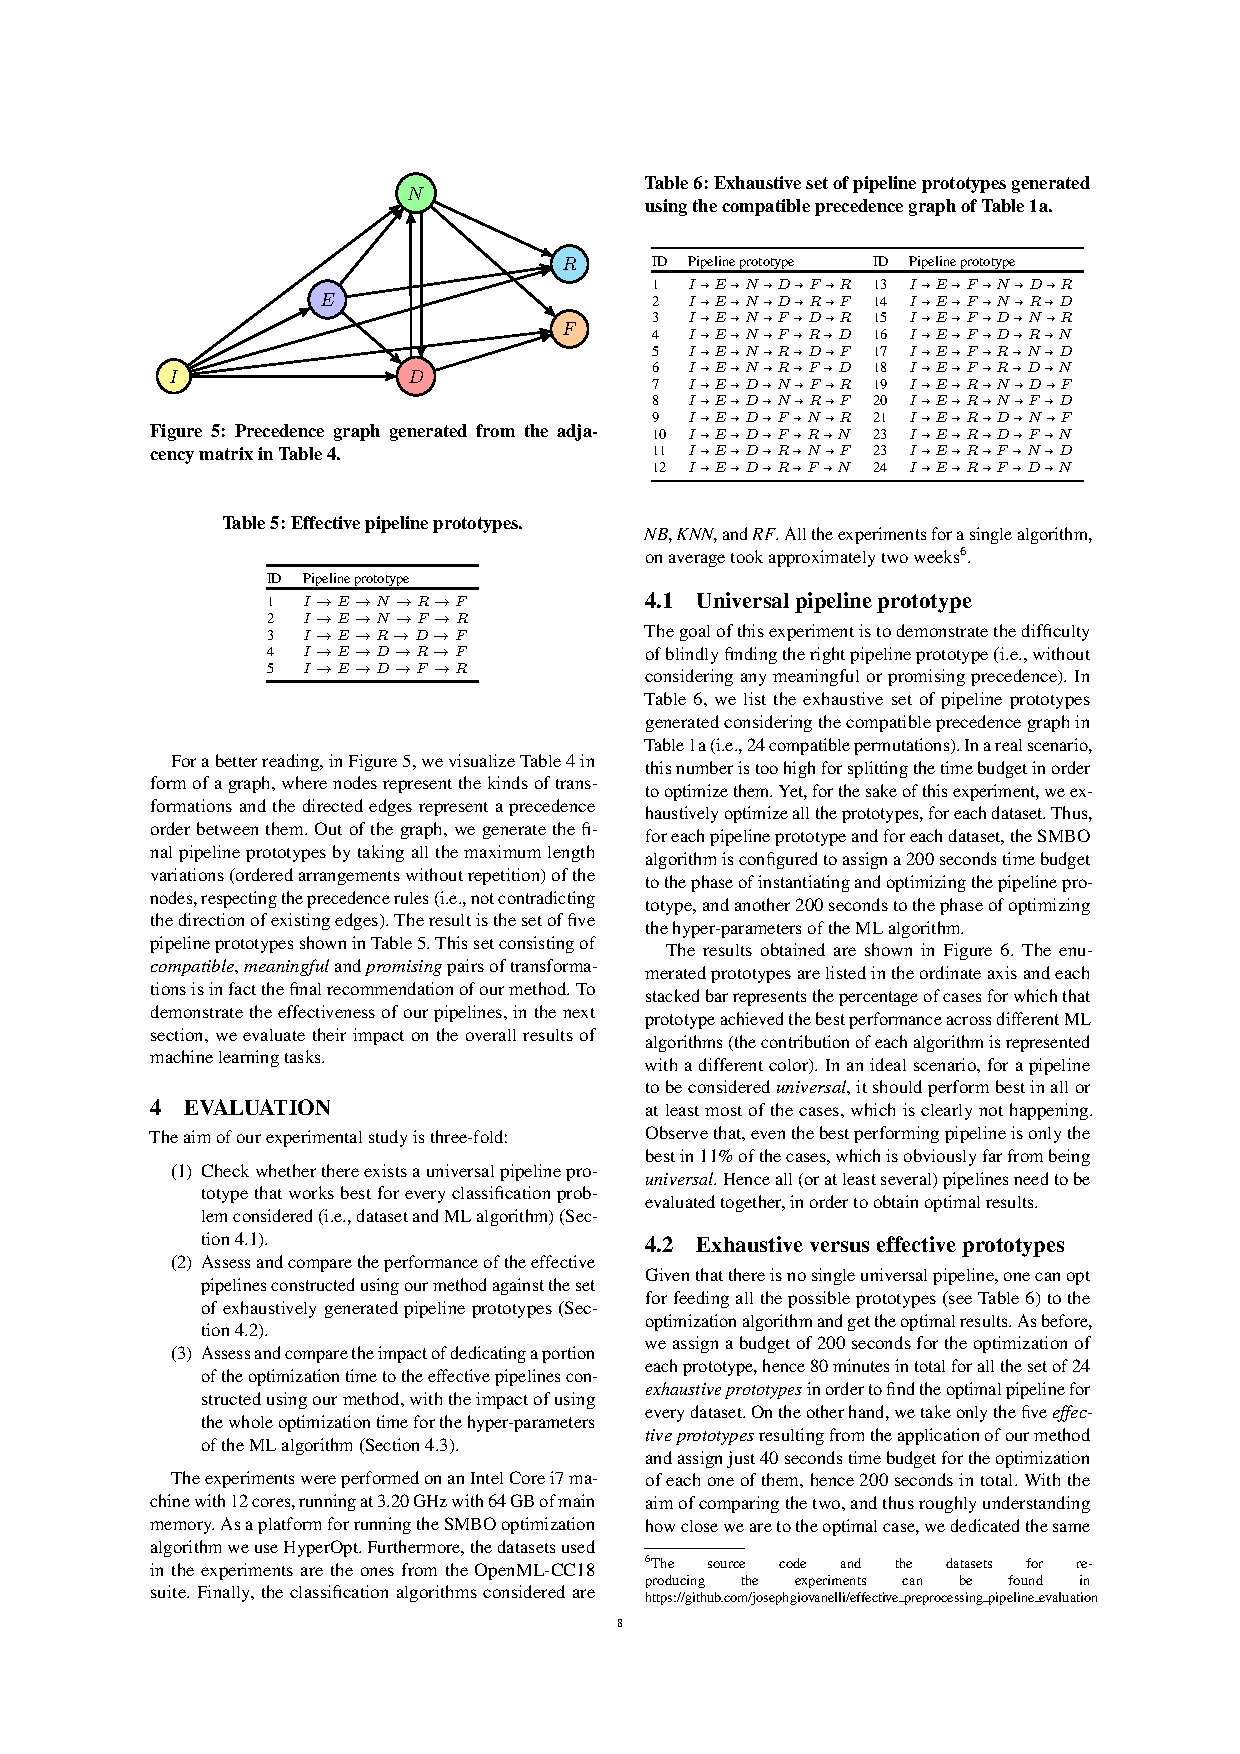
\includegraphics[clip, trim=2.5cm 23cm 10.5cm 2cm,width=0.5\textwidth]{chapters/data-centric/supervised/img/graph.pdf}
}{
  	\caption{Precedence graph generated from Table~\ref{tbl:rules-union}. $E$ - Encoding; $N$ - Normalization; $D$ - Discretization; $I$ - Imputation; $R$ - Rebalancing; $F$ - Feature Engineering. }
}
\capbtabbox{
\begin{tabular}{@{}ll}
			\toprule
			ID& Pipeline prototype                                             \\ \toprule
			1&{\color[HTML]{000000} $I\rightarrow E\rightarrow N \rightarrow R\rightarrow F$} \\
			2&{\color[HTML]{000000} $I\rightarrow E\rightarrow N \rightarrow F\rightarrow R$} \\
			3&{\color[HTML]{000000} $I\rightarrow E\rightarrow R \rightarrow D\rightarrow F$} \\
			4&{\color[HTML]{000000} $I\rightarrow E\rightarrow D \rightarrow R\rightarrow F$} \\
			5&{\color[HTML]{000000} $I\rightarrow E\rightarrow D \rightarrow F\rightarrow R$} \\
			\bottomrule
		\end{tabular}
}{
  	\caption{Effective pipeline prototypes generated from Figure~6. $E$ - Encoding; $N$ - Normalization; $D$ - Discretization; $I$ - Imputation; $R$ - Rebalancing; $F$ - Feature Engineering.
	}
}
\end{floatrow}
\end{figure}



\iffalse

\begin{figure}[t]
	\centering
	\begin{tikzpicture}[]
	\begin{scope}[xshift=10.5cm,yshift=-5cm,thick,
	node distance=1.0cm,on grid,>=stealth',
	block/.style={rectangle,draw,fill=cyan!20},
	vertex/.style={circle,draw,fill=orange!40},
	i/.style={circle,draw,fill=yellow!40},
	e/.style={circle,draw,fill=blue!25},
	f/.style={circle,draw,fill=orange!40},
	r/.style={circle,draw,fill=cyan!40},
	n/.style={circle,draw,fill=green!40},
	d/.style={circle,draw,fill=red!40}]
	decision/.style={diamond,draw,fill=white!40}]
	%layer0
	\node [i]	 (ti0) {$I$};
	\node [e]	 (te0)	[right=of ti0,xshift=1.6cm,yshift=1.3cm]	{$E$} edge [<-] (ti0);
	\node [n]	 (tn0)	[right=of te0,xshift=0.5cm,yshift=1.8cm]	{$N$} edge [<-] (te0);
	\node [d]	 (td0)	[right=of te0,xshift=0.5cm,yshift=-1.3cm]	{$D$} edge [<-] (te0);
	\node [r]	 (tr0)	[right=of tn0,xshift=1.6cm,yshift=-1.2cm]	{$R$} edge [<-] (tn0);
	\node [f]	 (tf0)	[right=of tn0,xshift=1.6cm,yshift=-2.3cm]	{$F$} edge [<-] (tn0);
	\path [->,draw,thick] (ti0) -- (tn0); 
	\path [->,draw,thick] (ti0) -- (tr0);
	\path [->,draw,thick] (ti0) -- (tf0);
	\path [->,draw,thick] (ti0) -- (td0);
	\path [->,draw,thick] (te0) -- (tr0);
	\path [->,draw,thick] (ti0) -- (tf0);
	\path [->,draw,thick] (td0) -- (tf0);
	\path [->,draw,thick] (tn0.285) -- (td0.75);
	\path [->,draw,thick] (td0.105) -- (tn0.255);
	\end{scope}
	\end{tikzpicture}
	\caption{Precedence graph generated from Table~\ref{tbl:rules-union}. $E$ - Encoding; $N$ - Normalization; $D$ - Discretization; $I$ - Imputation; $R$ - Rebalancing; $F$ - Feature Engineering.
	}
	\label{fig:precedence-graph}
\end{figure}


\begin{table}[t]
	\caption{Effective pipeline prototypes generated from Figure~6%\ref{fig:precedence-graph}
	. $E$ - Encoding; $N$ - Normalization; $D$ - Discretization; $I$ - Imputation; $R$ - Rebalancing; $F$ - Feature Engineering.
	}
	\footnotesize
	\label{tbl:effective-pipelines}
	\begin{center}
		\begin{tabular}{@{}ll}
			\toprule
			ID& Pipeline prototype                                             \\ \toprule
			1&{\color[HTML]{000000} $I\rightarrow E\rightarrow N \rightarrow R\rightarrow F$} \\
			2&{\color[HTML]{000000} $I\rightarrow E\rightarrow N \rightarrow F\rightarrow R$} \\
			3&{\color[HTML]{000000} $I\rightarrow E\rightarrow R \rightarrow D\rightarrow F$} \\
			4&{\color[HTML]{000000} $I\rightarrow E\rightarrow D \rightarrow R\rightarrow F$} \\
			5&{\color[HTML]{000000} $I\rightarrow E\rightarrow D \rightarrow F\rightarrow R$} \\
			\bottomrule
		\end{tabular}
	\end{center}
\end{table}
\fi

\end{example}
\subsection{Effective pipeline prototypes}
\label{sec:composition}
In this task we foresee the composition of the previously defined rules (i.e., for the pairs of transformations), to generate the final set of rules that would allow to compose longer chains --- consisting of more than two transformations. This is when we resolve the inconsistencies and also define precedences for the pairs of transformations that may not have any precedence defined already --- in that case, we basically take into account all the permutations. This step allows to finally generate the possible effective pipeline prototypes. 

\begin{example}
To generate the final pipeline prototypes, in this step we combine all the matrices generated by the previous steps. That is, we take the union of the edges (represented by \texttt{1}'s) from the matrices in Table~\ref{tbl:rules} (a,b,c), and create a new final adjacency matrix, shown in Table~\ref{tbl:rules-union}. This is the matrix that will allow us to generate the final effective pipeline prototypes. 

Observing the table, one can realize that for pairs $\{F,R\}$ and $\{R,D\}$, no precedence edges exist. This means that these pairs are somewhat equally relevant from either direction (any order), and thus when generating the final prototypes, both options should appear.

For a better reading, in Figure~6, we visualize Table~\ref{tbl:rules-union} in form of a graph, where nodes represent the kinds of transformations and the directed edges represent a precedence order between them.
Out of the graph, we generate the final pipeline prototypes by taking all the maximum length variations (ordered arrangements without repetition) of the nodes, respecting the precedence rules (i.e., not contradicting the direction of existing edges). The result is the set of five pipeline prototypes shown in Table 6. This set consisting of \textit{compatible}, \textit{meaningful} and \textit{promising} pairs of transformations is the set of recommended \textit{effective pipeline prototypes}.
\end{example}

\color{black}
\subsection{Meta-learning rules}
\label{sec:meta-learning}
Once the pipeline prototype is constructed, that is, the order between the kinds of transformations is defined, what follows is the instantiation of transformations with the physical operators. For that, one can rely completely on the optimization algorithm, and let the algorithm choose the right operators. However, given the way optimization algorithms work (e.g., SMBO) --- successively finding better and better instantiations, there is a cold-start problem, where in the beginning, the algorithm does not have enough information in order to come up with the most promising initial instantiations, and a wrong choice may affect the optimization process. 
\paragraph{Exploratory analysis}
Given the availability of the experimental SMBO executions (executed in an exhaustive manner, considering all the pipeline prototypes), one can perform an exploratory analysis with the aim of removing useless prototypes, pipelines or operators. Hence, further tweaking the search space. In particular, starting from the highest level, that of prototypes, then going to the physical pipelines, and finally to the actual operators inside the pipeline, one can analyze if:

\begin{itemize}
    \item there exist some combination of transformations in the form of prototypes (see Table~\ref{tbl:pipeline-enumeration} for the exhaustive list of prototypes), that are generally useless (i.e., in terms of their impact to the final accuracy), and thus can be discarded a priori in order to reduce the search space, 
    \item there are some physical pipelines that are consistently chosen more often than others by the optimization algorithm, meaning that they are more useful than others,
    \item within the physical pipelines, some transformations are chosen more often than others, meaning that they provide more positive impact. 
    \end{itemize}

\begin{example}
We performed the above-mentioned analysis to our use case, but it did not lead to any conclusive or significant results. In particular, as shown in Figure~\ref{fig:prototypes-impact}, we could not find any useless prototypes --- not positively impacting the final accuracy, that could be discarded a priori from the potential list of prototypes.
Actually, as we will show in Section~\ref{sec:eval-universal-pipeline}, all of them lead to the best in one case or another, which does not mean the epsilon improvement some provide is worth the search cost you incur in considering them (but this more in-depth analysis is done later).
Next, as shown in Figure~\ref{fig:pipeline-frequency}, there were no physical pipelines shown to be more useful --- hence more often selected, than others. Even if $N \rightarrow R$ is clearly above, it barely reaches 30\% in KNN.
 Finally, observing Figure~\ref{fig:transformation-frequency}, it is clear that some kinds of transformations are chosen more often, but looking closely (i.e., the shaded bars), it is not clear which operator brings more benefit. For instance, Normalization is present in 90\% of the pipelines, but it is not easy to distinguish which kind of Normalization (i.e., actual operator) is more beneficial.
For this, we need more complex rules or guidelines that may help in finding the right operator to use. 
\end{example}

\begin{figure*}[!t]
	\centering
	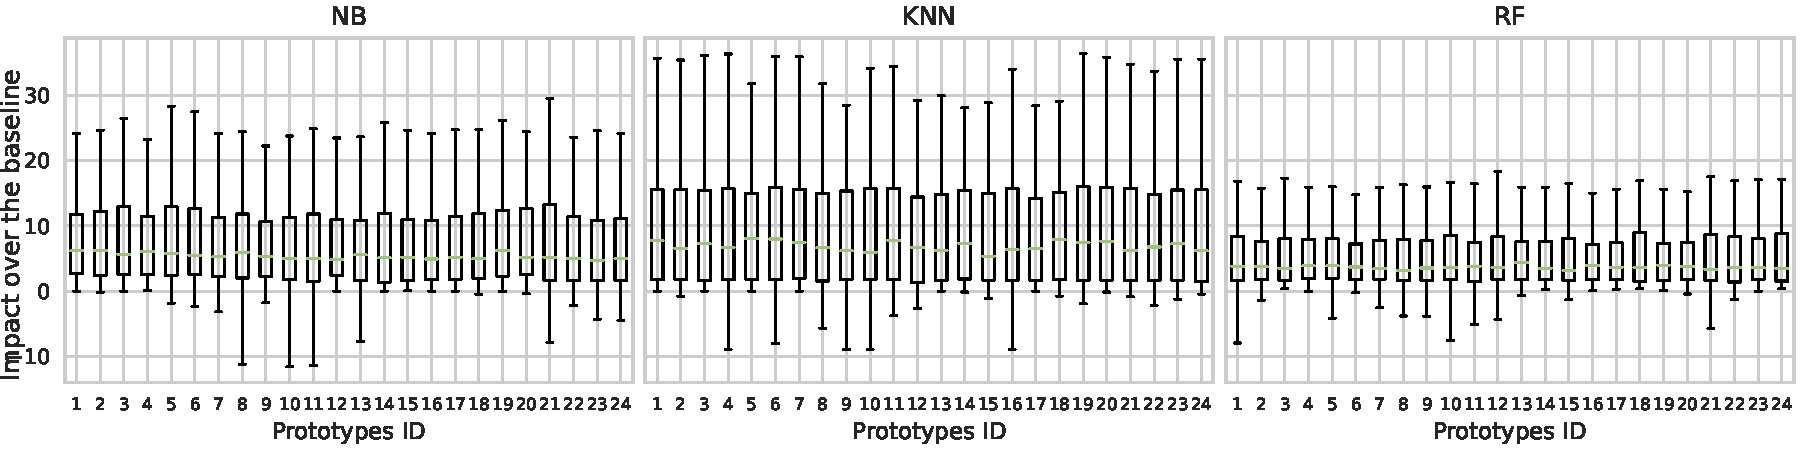
\includegraphics[width=1.0\textwidth]{chapters/data-centric/supervised/img/prototypes_impact.pdf}
	\caption{The impact of the different pipeline prototypes over the baseline (i.e., when no transformation is applied).}
	\label{fig:prototypes-impact}
\end{figure*}

\begin{figure*}[!h]
	\centering
	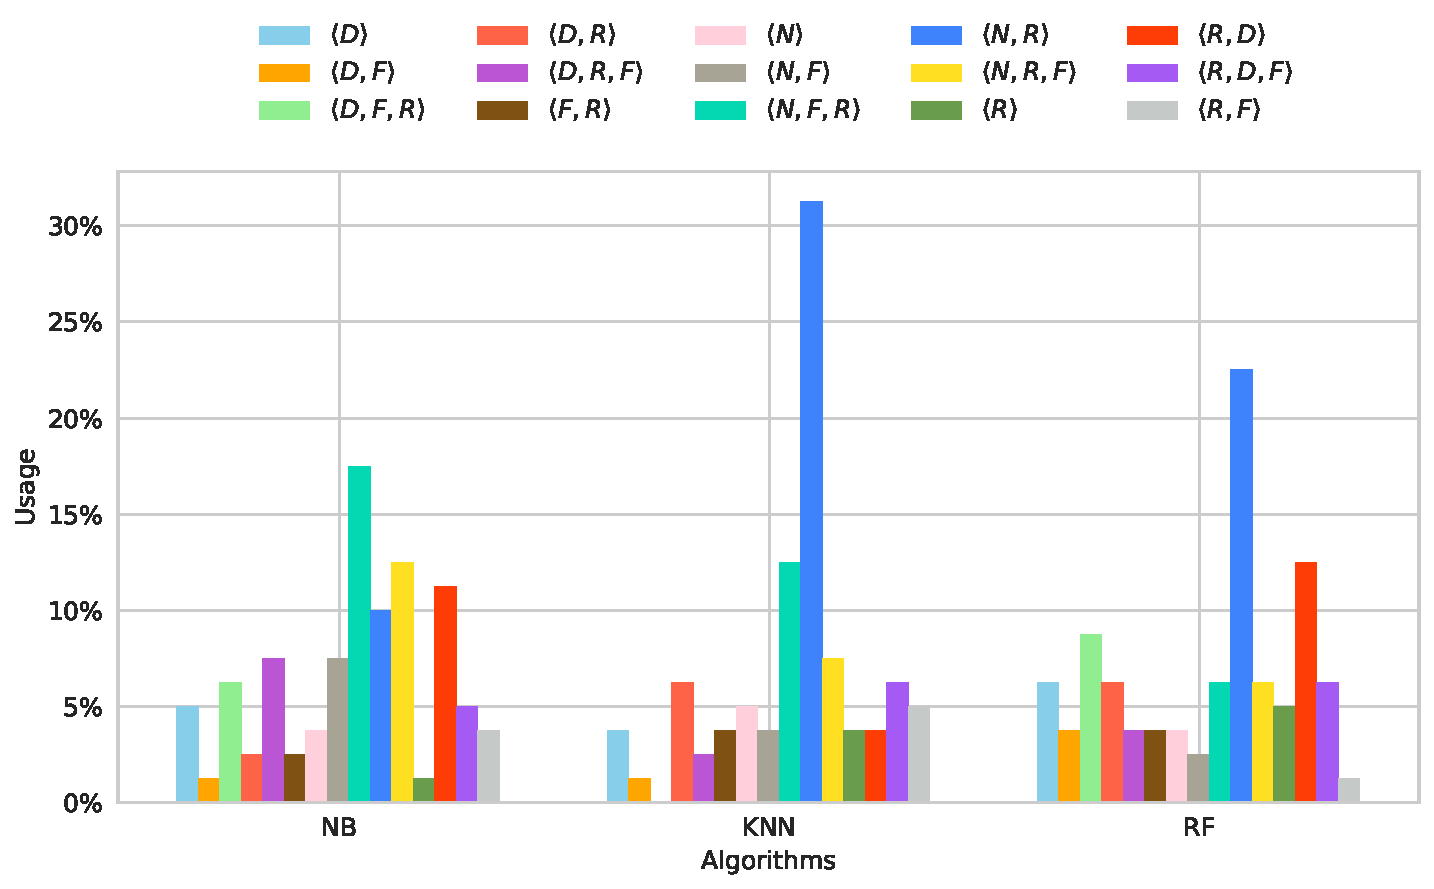
\includegraphics[width=1.0\textwidth]{chapters/data-centric/supervised/img/pp_pipeline_study2.pdf}
	\caption{Percentage of use of the different physical pipelines.}
	\label{fig:pipeline-frequency}
\end{figure*}

\begin{figure*}[!h]
	\centering
	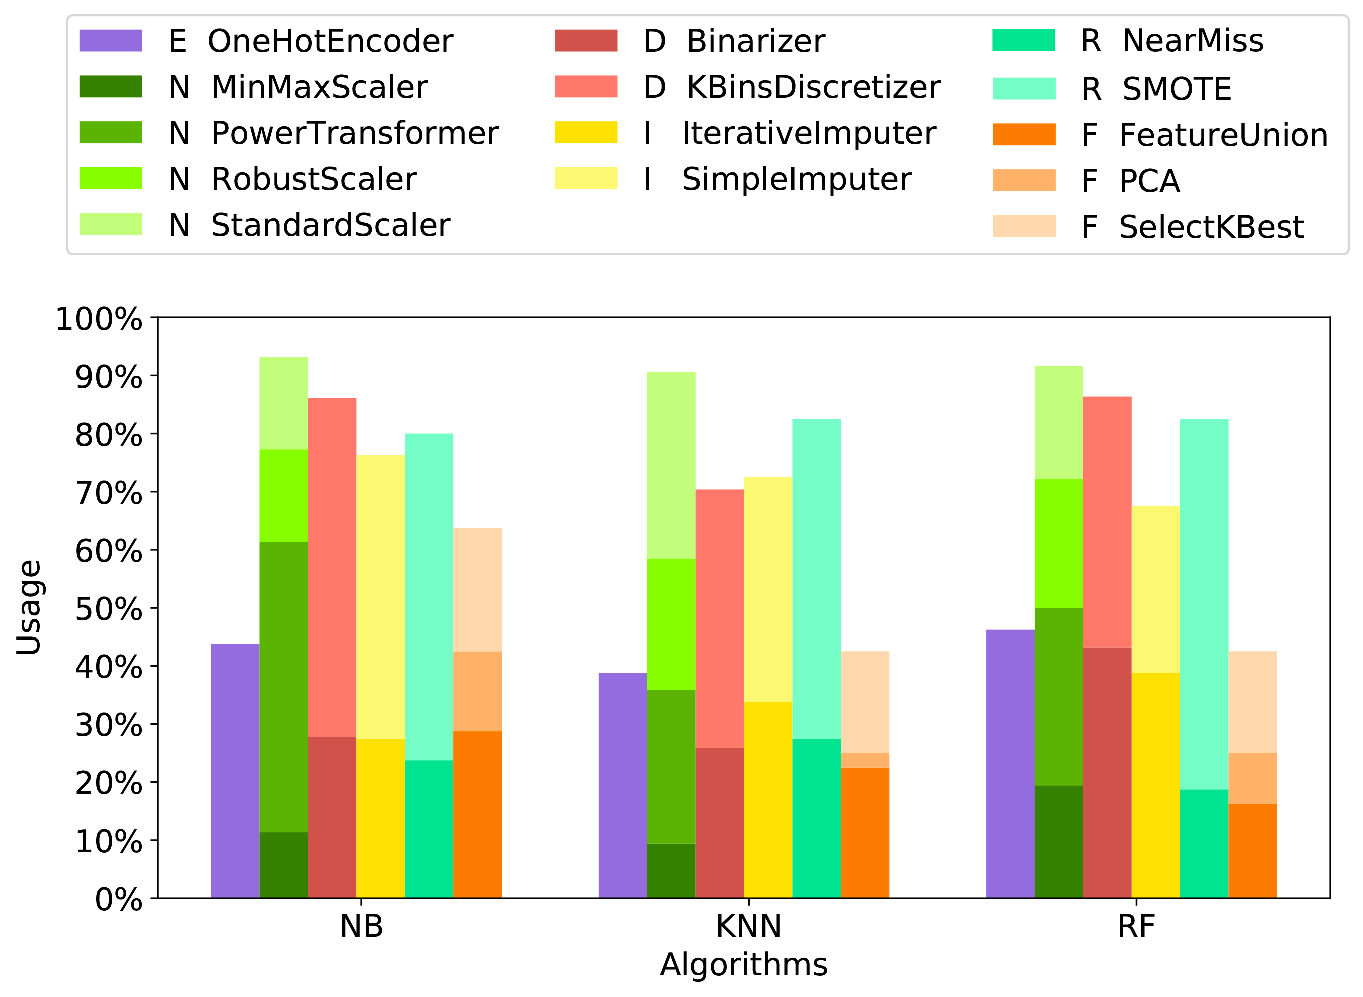
\includegraphics[width=0.7\textwidth]{chapters/data-centric/supervised/img/pp_pipeline_study_grouped.pdf}
	\caption{Percentage of use of a transformation in a physical pipeline.}
	\label{fig:transformation-frequency}
\end{figure*}

\subsection{Meta-learning}
\color{black}
To mitigate the red cold-start problem, we propose to perform meta-learning (shown in Figure~\ref{fig:methodology}), where we intend to use the knowledge extracted from historical data in order to devise rules that may help the optimization algorithm in its initial phase. 
Meta-learning is the process of `learning on top of learning', or learning a model using historical data from ML experiments. Traditionally, it has been used for predicting the performance (e.g., predictive accuracy) of an algorithm on a given dataset. That is, given some historical runs of the performance of classification algorithms over various datasets (i.e., meta-database: consisting of datasets characteristics as predictive variables and the performance of the classification algorithm as the response variable), one can learn a model (i.e., meta-model), that is able to predict the performance of a given classification algorithm on a new dataset~\cite{Brazdil04Book}. Lately, this technique has been extended in order to predict the impact of transformations over the performance of classification algorithms and thus rank transformations based on their impact~\cite{Bilalli17AMCS, presistant18CSI, presistant19DKE}. The same idea can be applied for learning the best operator for a given transformation.
That is, through meta-learning one can learn the intrinsic relationship between dataset characteristics and the operator performance, and thus come up with rules that are not obvious and are effective at the time of instantiating a transformation. 
The main idea is to build a model, that is able to predict the operator for a certain kind of transformation, given the meta-features extracted from the dataset considered for the optimization. This translates to answering the following question: ``given that we know the dataset characteristics and having selected a certain kind of transformation (e.g., missing value imputation), what is the optimal physical algorithm (see Table~\ref{tbl:transformations}) we need to select, to obtain the highest improvement possible in terms of classification accuracy (i.e., when the classification algorithm is applied over the transformed dataset)?".  In particular, the model can generate a set of complementary rules that help in the optimization, providing a good starting instantiation for some of the transformations in the prototype.

To train the model we need a meta-dataset that can be  (i) generated through optimization algorithms (e.g., SMBO executions), (ii) generated manually through simple evaluations of classification algorithms over transformed datasets, or (iii) assumed already given (e.g., OpenML). 

Given a meta-dataset, we propose to learn to predict the best instantiation (operator) for a given transformation, where among the classes we can include the class \texttt{None} too. This means that one of the possible predictions is to not instantiate a transformation at all, hence remove it from the pipeline.

\begin{example}
Our training dataset (sometimes referred to as `meta-database' or `meta-dataset') for the meta-learning is compiled through SMBO runs on the OpenML datasets (see Section~\ref{sec:rules-learned:algorithm}). That is, we first extract the dataset characteristics/profiles (i.e., number of features, number of instances, number of missing values, etc), and then by applying SMBO optimization, on classification algorithms and pre-processing pipelines (as explained in Section~\ref{sec:composition}), for each dataset, we retrieve the evaluations (i.e., predictive accuracy) of the algorithms over the optimized pipelines. This gives us the presumably optimal physical pipelines and their impact on the accuracy of the learning algorithms for each dataset at hand. Given such information, our aim is to now save time and improve the instantiation of the operators for each transformation considered in the prototype. 

We trained several different Conditional Inference Trees \cite{ctree} because they produce models that can be easily read and interpreted.
Specifically, the independence of each variable (meta-features in our case) with the class (operator of a specific transformation) is tested through a statistical test. 
The split is made on the variable with the lowest p-value. 
We report the p-value too, so that it can be seen how strong the association is (i.e., why that variable was chosen).
We stick with the p-value threshold of 0.05, and devise a rule from any branch of the tree that is within the threshold. In the following, we describe the rules obtained within the selected significance threshold.

\textbf{Rules for Feature Engineering}. The available operators in Scikit-learn for Feature Engineering (see Table~\ref{tbl:transformations}) are: \texttt{PCA} (Principal Component Analysis), \texttt{Feature Selection} (Select K Best), \texttt{Both} (PCA + Select K Best), and \texttt{None}. The tree generated for the Feature Engineering transformation is shown in Figure~\ref{fig:features-meta-learning:feature-engineering}. The leaves show the selected operator frequency. For the sake of simplicity, we do not consider the union of PCA and Select K Best as an operator per se, instead we distribute that contribution to the two operators that compose it.
Observe that there is a strong correlation between the Feature Engineering operator and the entropy of the class attribute.
Indeed, such a meta-feature achieved a p-value smaller than 0.001.
We can clearly read that if the Class Entropy is low, then \texttt{Feature Selection} is way more chosen than the other options (see Node 2).
Recall that the entropy of an attribute is a measure of how much disorder there is among its instances.
The less is that value, the easier is the classification problem.
As a consequence, it is reasonable to think that the easier the classification problem is, the more likely is the fact that the class can be described by a low number of features.
Hence, the \texttt{Feature Selection} technique can be successfully applied.
Conversely, Node 5 shows that, when the Class Entropy is high, it is better to not apply any Feature Engineering operator.
As a matter of fact, a high value of Class Entropy involves a high number of classes and/or few instances per class, hence a really difficult problem.
In such cases, reducing the dimensionality of the dataset does not lead to any improvement.
Finally, when the Class Entropy is in between, there is no clear winner, and thus other non-obvious factors may affect the choice of the operator.

\textbf{Rules for Rebalancing}. As for Rebalancing, the operators considered from the imblearn\footnote{\url{https://pypi.org/project/imbalanced-learn}} library are: \texttt{Near Miss}, \texttt{SMOTE}, and \texttt{None}. %\joseph{the rebalance implementations are of actually from imblearn (imbalanced-learn)}
The first is an undersampling algorithm which randomly eliminates the samples from the larger class.
Instead, the second is an oversampling technique that creates samples of the minority class, as a linear combination of them.
As shown in Figure~\ref{fig:features-meta-learning:rebalancing}, the meta-feature Majority Class Percentage has a p-value of 0.014.
This can be read as, in case of an unbalanced class problem (i.e., Node 3: Majority Class Percentage greater than 56), an oversampling of the minority class(es) is preferred to a downsampling of the majority one(s).
However, when the Majority Class Percentage is smaller than 56\%, the situation is not that clear, and there is no technique that is applied significantly more often than the rest; they are close to each other.
Therefore, it is difficult to understand which problems (which dataset characteristics do they have) belong to Node 2.
In summary, when the majority class has no more than 56\% , it implies that it is an unbalanced class, and as mentioned above, SMBO tends to choose the same operator. However, when the majority class has less than 56\%, it may imply that: (i) there are just two classes and the problem counts as a balanced problem, so no operator needs to be applied, or (ii) it is a multi-class problem, and thus there is no clear winner in terms of operators. 
\end{example}


\subsection{Prototype instantiation}

The prototypes from the top flow and the meta-lerning rules from the bottom flow (if the optimization framework permits), are finally fed to the final step which deals with the instantiation and optimization of the prototypes. In this task we run an optimization algorithm that is executed until an optimal pipeline is found.

\begin{example}
 In our final execution, we run SMBO to find a suitable instantiation for the suggested prototypes. The simple but not obvious meta-learning rules, even though not included in our final execution, because of the implementation considered (i.e., HyperOpt), can potentially be used to ease the cold-start problem. 
\end{example}

\begin{figure*}[!h]
	\centering
	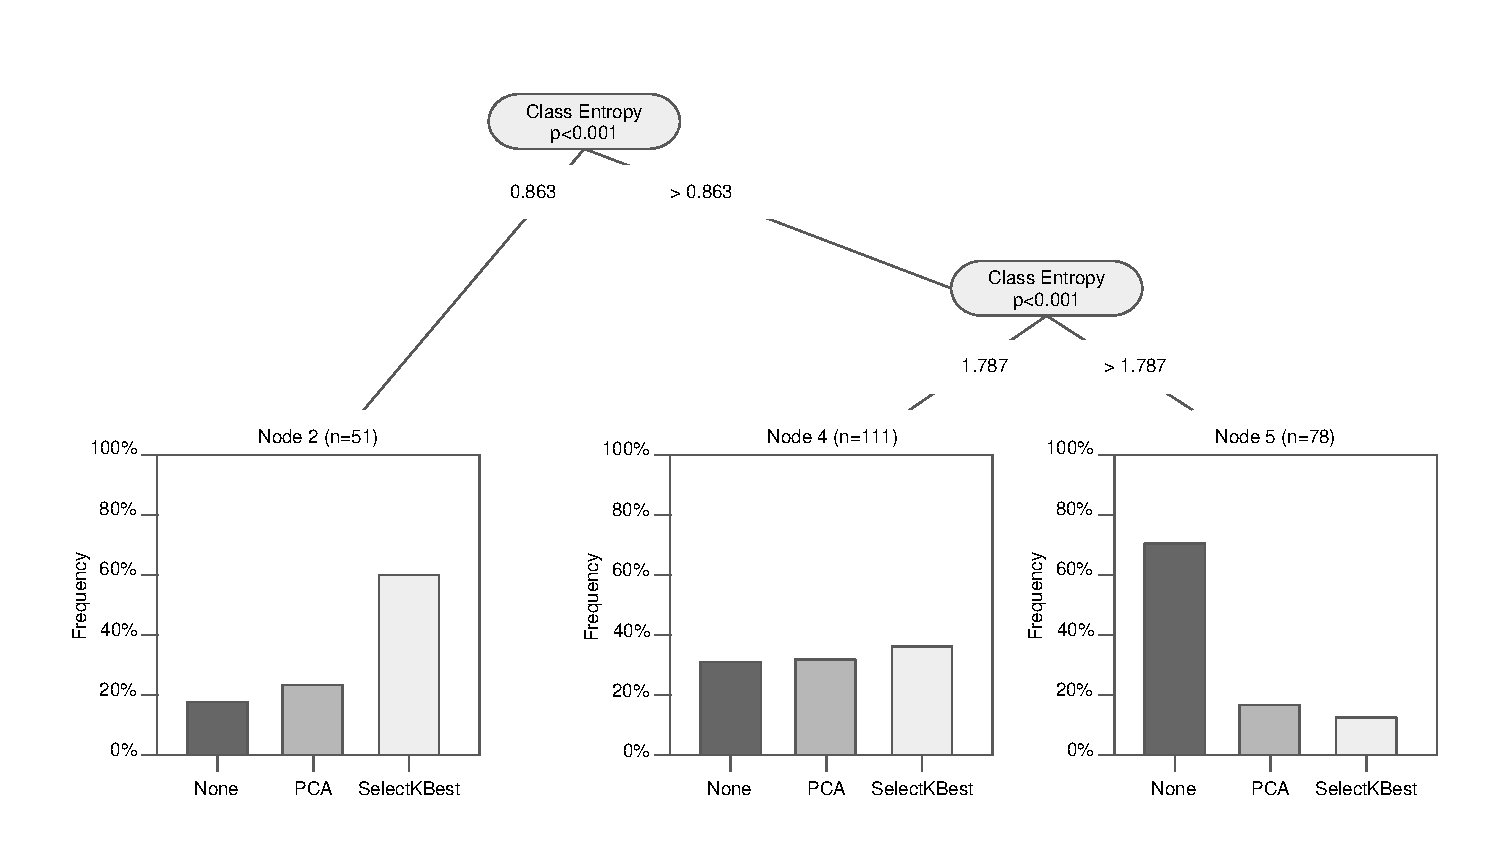
\includegraphics[clip, trim=1.0cm 0.4cm 1cm 1cm,width=1\textwidth]{chapters/data-centric/supervised/img/tree-FE.pdf}
	\caption{Conditional Inference Tree built for the \textit{Features Engineering} transformation.}
	\label{fig:features-meta-learning:feature-engineering}
\end{figure*}

\begin{figure*}[!h]
	\centering
	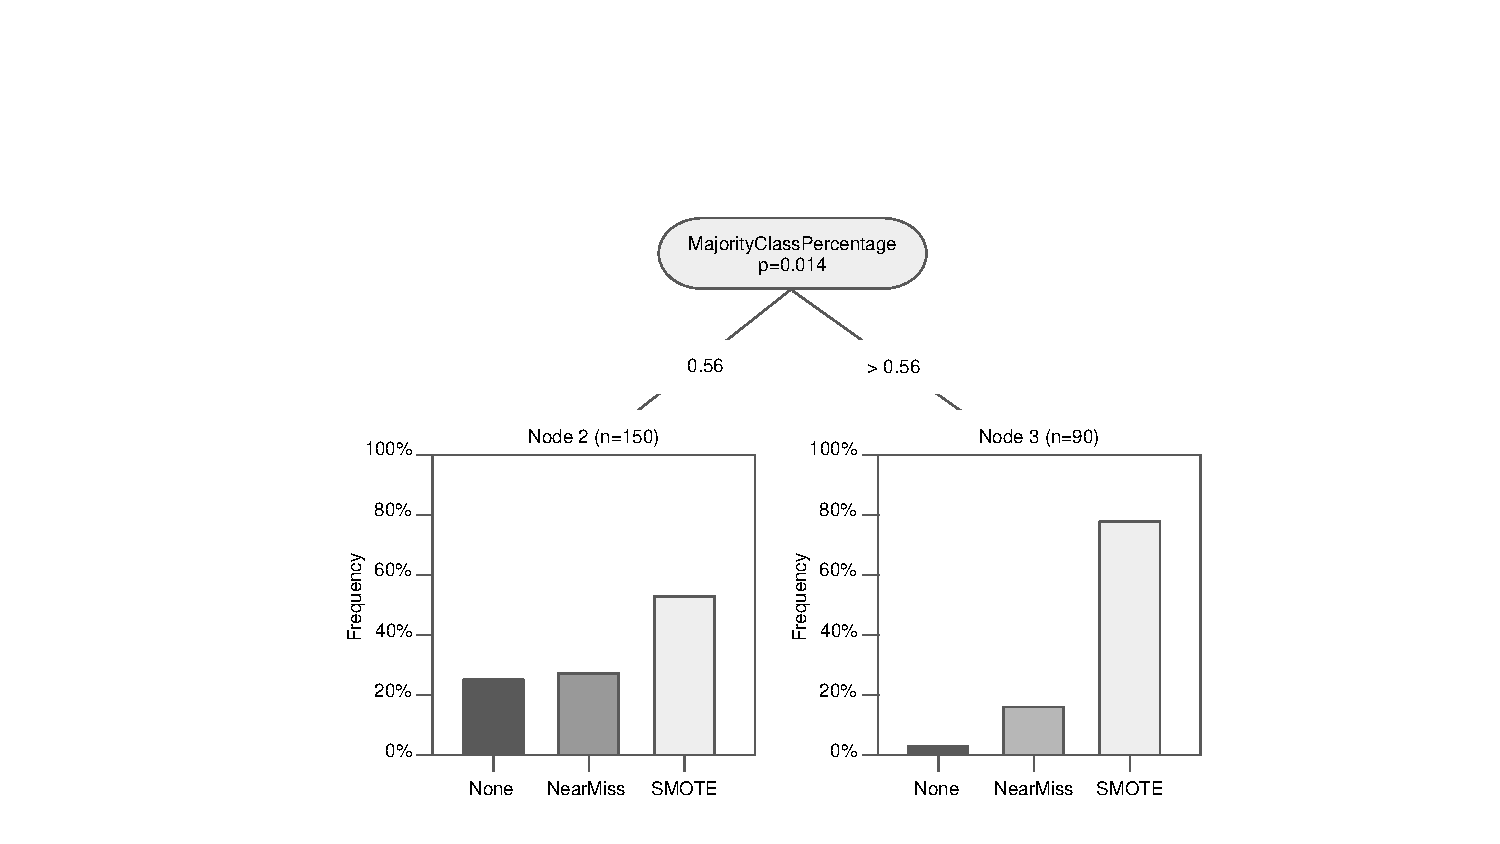
\includegraphics[clip, trim=5.8cm 0.4cm 5.05cm 3.5cm,width=0.65\textwidth]{chapters/data-centric/supervised/img/tree-RE.pdf}
	\caption{Conditional Inference Tree built for the \textit{Rebalancing} transformation.}
	\label{fig:features-meta-learning:rebalancing}
	\end{figure*}

%In our recent future work we aim to extend HyperOpt with the functionality of incorporating mechanisms that ease the cold start problem. The technique of using meta-learning for the cold-start problem has for instance been applied in \cite{Feurer15AAAI}, however the overall method lacks the initial part of finding promising pipeline prototypes (i.e., works over single transformations), meaning that the instantiation via meta-learning may occur in the wrong place (not the optimal prototype), resulting into a solution that is a local optimum. 


\section{Evaluation}
\label{sec:evaluation}

The aim of our experimental study is three-fold:
\begin{enumerate}
    \item Check whether there exists a universal pipeline prototype that works best for any classification problem considered  (i.e., dataset and ML algorithm) (Section~\ref{sec:eval-universal-pipeline}).
    \item Assess and compare the performance of the effective pipelines constructed using our method against the set of exhaustively generated pipeline prototypes (Section~\ref{sec:eval-our-vs-rest}).
    \item Assess and compare the impact of dedicating a portion of the optimization time to the effective pipelines constructed using our method, with the impact of using the whole optimization time for the hyper-parameters of the ML algorithm (Section~\ref{sec:eval-dpso-vs-cash}).
\end{enumerate}

The experiments were performed on an Intel Core i7 machine with 12 cores, running at 3.20 GHz with 64 GB of main memory. As a platform for running the SMBO optimization algorithm we use HyperOpt. Furthermore, the datasets used in the experiments are the ones from the OpenML repository (see Section~\ref{sec:rules-learned:algorithm}). Finally, the classification algorithms considered are \textit{NB}, \textit{KNN}, and \textit{RF}. All the experiments for a single algorithm, on average took approximately two weeks\footnote{The source code and the datasets for reproducing the experiments can be found in 
\href{https://github.com/josephgiovanelli/effective\_preprocessing\_pipeline\_evaluation}{https://github.com/josephgiovanelli/effective\_preprocessing\_pipeline\_evaluation}}.

\subsection{Universal pipeline prototype}
\label{sec:eval-universal-pipeline}
The goal of this experiment is to demonstrate the difficulty of blindly finding the right pipeline prototype (i.e., without considering any meaningful or promising precedence).
In Table~\ref{tbl:pipeline-enumeration}, we list the exhaustive set of pipeline prototypes generated considering the compatible precedence graph in Table~\ref{tbl:rules}a (i.e., 24 compatible permutations). In a real scenario, this number would be too high for splitting the time budget in order to optimize them. 
Yet, for the sake of this experiment, we exhaustively optimize all the prototypes, for each dataset. Thus, for each pipeline prototype and for each dataset, the SMBO algorithm is configured to assign a 200 seconds time budget to the phase of instantiating and optimizing the pipeline prototype, and another 200 seconds to the phase of optimizing the hyper-parameters of the ML algorithm.

\begin{table}[t]
\caption[Enumeration of the pipelines that can be generated by compatible precedence]{Exhaustive set of pipeline prototypes generated using the compatible precedence graph of Table~\ref{tbl:rules}a. $E$ - Encoding; $N$ - Normalization; $D$ - Discretization; $I$ - Imputation; $R$ - Rebalancing; $F$ - Feature Engineering.
}
\footnotesize
\label{tbl:pipeline-enumeration}
\begin{center}
\begin{tabular}{@{}lllll@{}}
\toprule
ID & Pipeline prototype & ID & Pipeline prototype                                                                   \\ \toprule
1  & {\color[HTML]{000000} $I\veryshortarrow E\veryshortarrow N \veryshortarrow D\veryshortarrow F \veryshortarrow R$} & 13 & {\color[HTML]{000000} $I\veryshortarrow E \veryshortarrow F \veryshortarrow N \veryshortarrow D\veryshortarrow R$} \\
2  & {\color[HTML]{000000} $I\veryshortarrow E\veryshortarrow N \veryshortarrow D\veryshortarrow R \veryshortarrow F$} & 14 & {\color[HTML]{000000} $I\veryshortarrow E \veryshortarrow F \veryshortarrow N \veryshortarrow R \veryshortarrow D$} \\
3  & {\color[HTML]{000000} $I\veryshortarrow E\veryshortarrow N \veryshortarrow F \veryshortarrow D\veryshortarrow R$} & 15 & {\color[HTML]{000000} $I\veryshortarrow E \veryshortarrow F \veryshortarrow D\veryshortarrow N \veryshortarrow R$} \\
4  & {\color[HTML]{000000} $I\veryshortarrow E\veryshortarrow N \veryshortarrow F \veryshortarrow R \veryshortarrow D$} & 16 & {\color[HTML]{000000} $I\veryshortarrow E \veryshortarrow F \veryshortarrow D\veryshortarrow R \veryshortarrow N$} \\
5  & {\color[HTML]{000000} $I\veryshortarrow E\veryshortarrow N \veryshortarrow R \veryshortarrow D\veryshortarrow F$} & 17 & {\color[HTML]{000000} $I\veryshortarrow E \veryshortarrow F \veryshortarrow R \veryshortarrow N \veryshortarrow D$} \\
6  & {\color[HTML]{000000} $I\veryshortarrow E\veryshortarrow N \veryshortarrow R \veryshortarrow F \veryshortarrow D$} & 18 & {\color[HTML]{000000} $I\veryshortarrow E \veryshortarrow F \veryshortarrow R \veryshortarrow D\veryshortarrow N$} \\
7  & {\color[HTML]{000000} $I\veryshortarrow E \veryshortarrow D\veryshortarrow N \veryshortarrow F \veryshortarrow R$} & 19 & {\color[HTML]{000000} $I\veryshortarrow E \veryshortarrow R \veryshortarrow N \veryshortarrow D \veryshortarrow F$} \\
8  & {\color[HTML]{000000} $I\veryshortarrow E \veryshortarrow D\veryshortarrow N \veryshortarrow R \veryshortarrow F$} & 20 & {\color[HTML]{000000} $I\veryshortarrow E \veryshortarrow R \veryshortarrow N \veryshortarrow F \veryshortarrow D$} \\
9  & {\color[HTML]{000000} $I\veryshortarrow E \veryshortarrow D\veryshortarrow F\veryshortarrow N \veryshortarrow R$} & 21 & {\color[HTML]{000000} $I\veryshortarrow E \veryshortarrow R \veryshortarrow D\veryshortarrow N \veryshortarrow F$} \\
10 & {\color[HTML]{000000} $I\veryshortarrow E \veryshortarrow D\veryshortarrow F \veryshortarrow R\veryshortarrow N$} & 23 & {\color[HTML]{000000} $I\veryshortarrow E \veryshortarrow R \veryshortarrow D \veryshortarrow F \veryshortarrow N$} \\
11 & {\color[HTML]{000000} $I\veryshortarrow E \veryshortarrow D\veryshortarrow R \veryshortarrow N \veryshortarrow F$} & 23 & {\color[HTML]{000000} $I\veryshortarrow E \veryshortarrow R \veryshortarrow F \veryshortarrow N \veryshortarrow D$} \\
12 & {\color[HTML]{000000} $I\veryshortarrow E \veryshortarrow D\veryshortarrow R \veryshortarrow F\veryshortarrow N$} & 24 & {\color[HTML]{000000} $I\veryshortarrow E \veryshortarrow R \veryshortarrow F \veryshortarrow D\veryshortarrow N$}
\\ \bottomrule
\end{tabular}
\end{center}
\end{table}

The results obtained are shown in Figure~\ref{fig:eval-universal-pipeline}.
The enumerated prototypes are listed in the ordinate axis and each stacked bar represents the percentage of cases for which that prototype achieved the best performance across different ML algorithms (the contribution of each algorithm is represented with a different color). In an ideal scenario, for a pipeline to be considered \textit{universal}, it should perform best in all or at least most of the cases, which is clearly not happening. Observe that, even the best performing pipeline is only the best in 19\% of the cases, which is obviously far from being \textit{universal}. Hence all (or at least several) pipelines need to be evaluated together, in order to obtain better solutions. 

\begin{figure}[t]
    \centering
    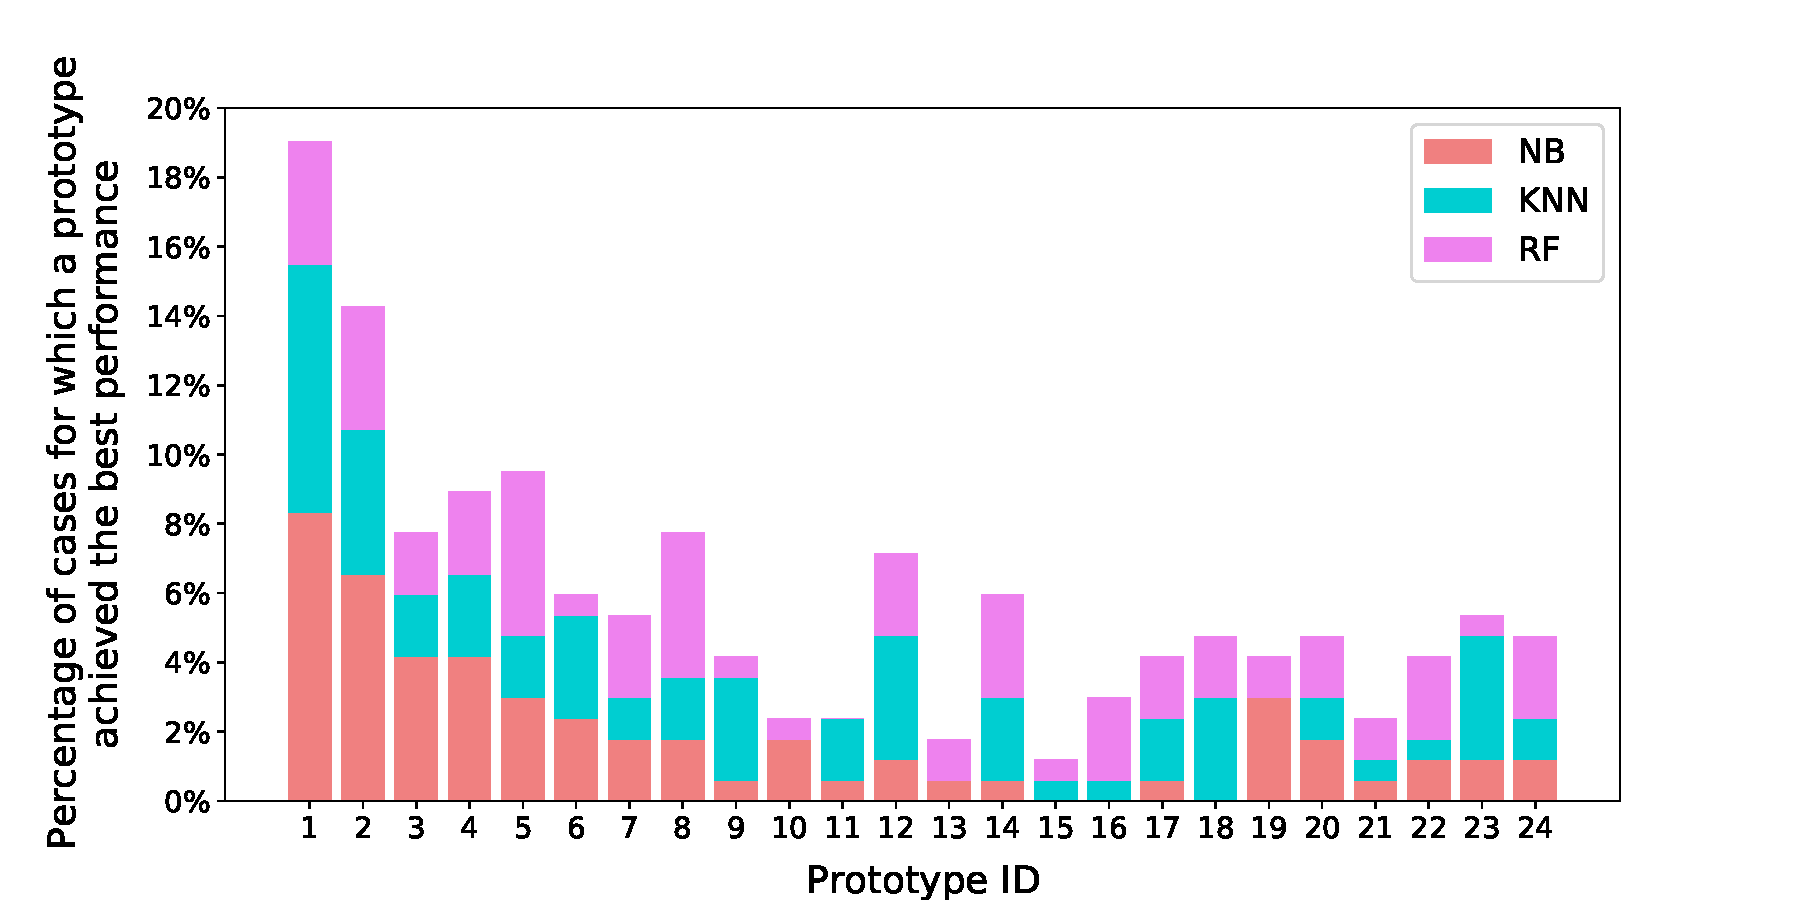
\includegraphics[width=0.8\textwidth]{chapters/data-centric/supervised/img/evaluation1.pdf}
    \caption{Comparison of the goodness of the exhaustive set of prototypes.}
    \label{fig:eval-universal-pipeline}
\end{figure}

\subsection{Exhaustive versus effective prototypes}
\label{sec:eval-our-vs-rest}
Given that there is no single universal pipeline, one can opt for feeding all the possible prototypes (see Table~\ref{tbl:pipeline-enumeration}) to the optimization algorithm in order to get the best solutions out of them. 
As before, we assign a budget of 200 seconds for the optimization of each prototype, hence 80 minutes in total for all the set of 24 \textit{exhaustive prototypes} in order to find the optimal pipeline for every dataset. On the other hand, we take only the five \textit{effective prototypes} resulting from the application of our method and assign just 40 seconds time budget for the optimization of each one of them, hence 200 seconds in total. With the aim of comparing the two, and thus roughly understanding how close we are to the optimal case, in both cases, we dedicated the same time budget (i.e., 200 seconds) for the phase of optimizing the hyper-parameters of the ML algorithm.
In order to evaluate how close the \textit{effective prototypes} are to the \textit{exhaustive ones}, we calculate the \textit{normalized distance} from the result to the optimum:

\begin{equation*}
    normalized\;distance = \frac{Acc(d_{e\!f\!f\!ective},a^*) - Acc(d,a)}{Acc(d_{exhaustive},a^*) - Acc(d,a)}
\end{equation*}

where, $Acc(d,a)$ is the baseline performance (i.e., predictive accuracy of the algorithm $a$ with default hyper-parameters over the original dataset $d$). $Acc(d_{e\!f\!f\!ective},a^*)$ is the accuracy of the optimized algorithm $a^*$ over the dataset $d_{e\!f\!f\!ective}$ transformed using the optimized instantiation of the effective set of prototypes (i.e., our approach). Finally, ~$Acc(d_{exhaustive},a^*)$ is the accuracy of the optimized algorithm $a^*$ over the dataset $d_{exhaustive}$ transformed using the optimized pipeline instantiation of the exhaustive set of prototypes. The subtraction by $Acc(d,a)$ is done with the aim of weighting the difficulty of a dataset, hence allowing for comparisons in terms of the gain in accuracy. To this end, the bigger the potential gain (denominator) is, the bigger the obtained gain (numerator) must be, for the latter to be relevant. 

The results obtained for every dataset and algorithm are shown as boxplots in Figure~\ref{fig:eval-exhaustive-vs-effective}. Observe that, most of the cases are very close to the results obtained using the exhaustive set, the median distances being 91.51\%, 93.13\%, 88.97\%, for NB, KNN, and RF, respectively. 
In general, in 75\% of the cases the chosen pipelines are above 80\%, and only few outliers are below 60\%. Curiously, in some cases, we outperform the results over the exhaustive set of pipelines, but this is due to the randomness of the optimization algorithm, which unless it is given an unrealistically high budget of time, is not capable of finding the true optimal solution. We discarded the option of assigning a larger budget since this was not practical considering the huge search space and the lack of any guarantee of improvement. 

To summarize, the experiment shows that with roughly 24 times less time budget, we can obtain results that are as good as 90\% in the median compared to the exhaustive ones. The raw results (i.e., without the normalized distances) can be found on the aforementioned github page.

\begin{figure}[!t]
    \centering
    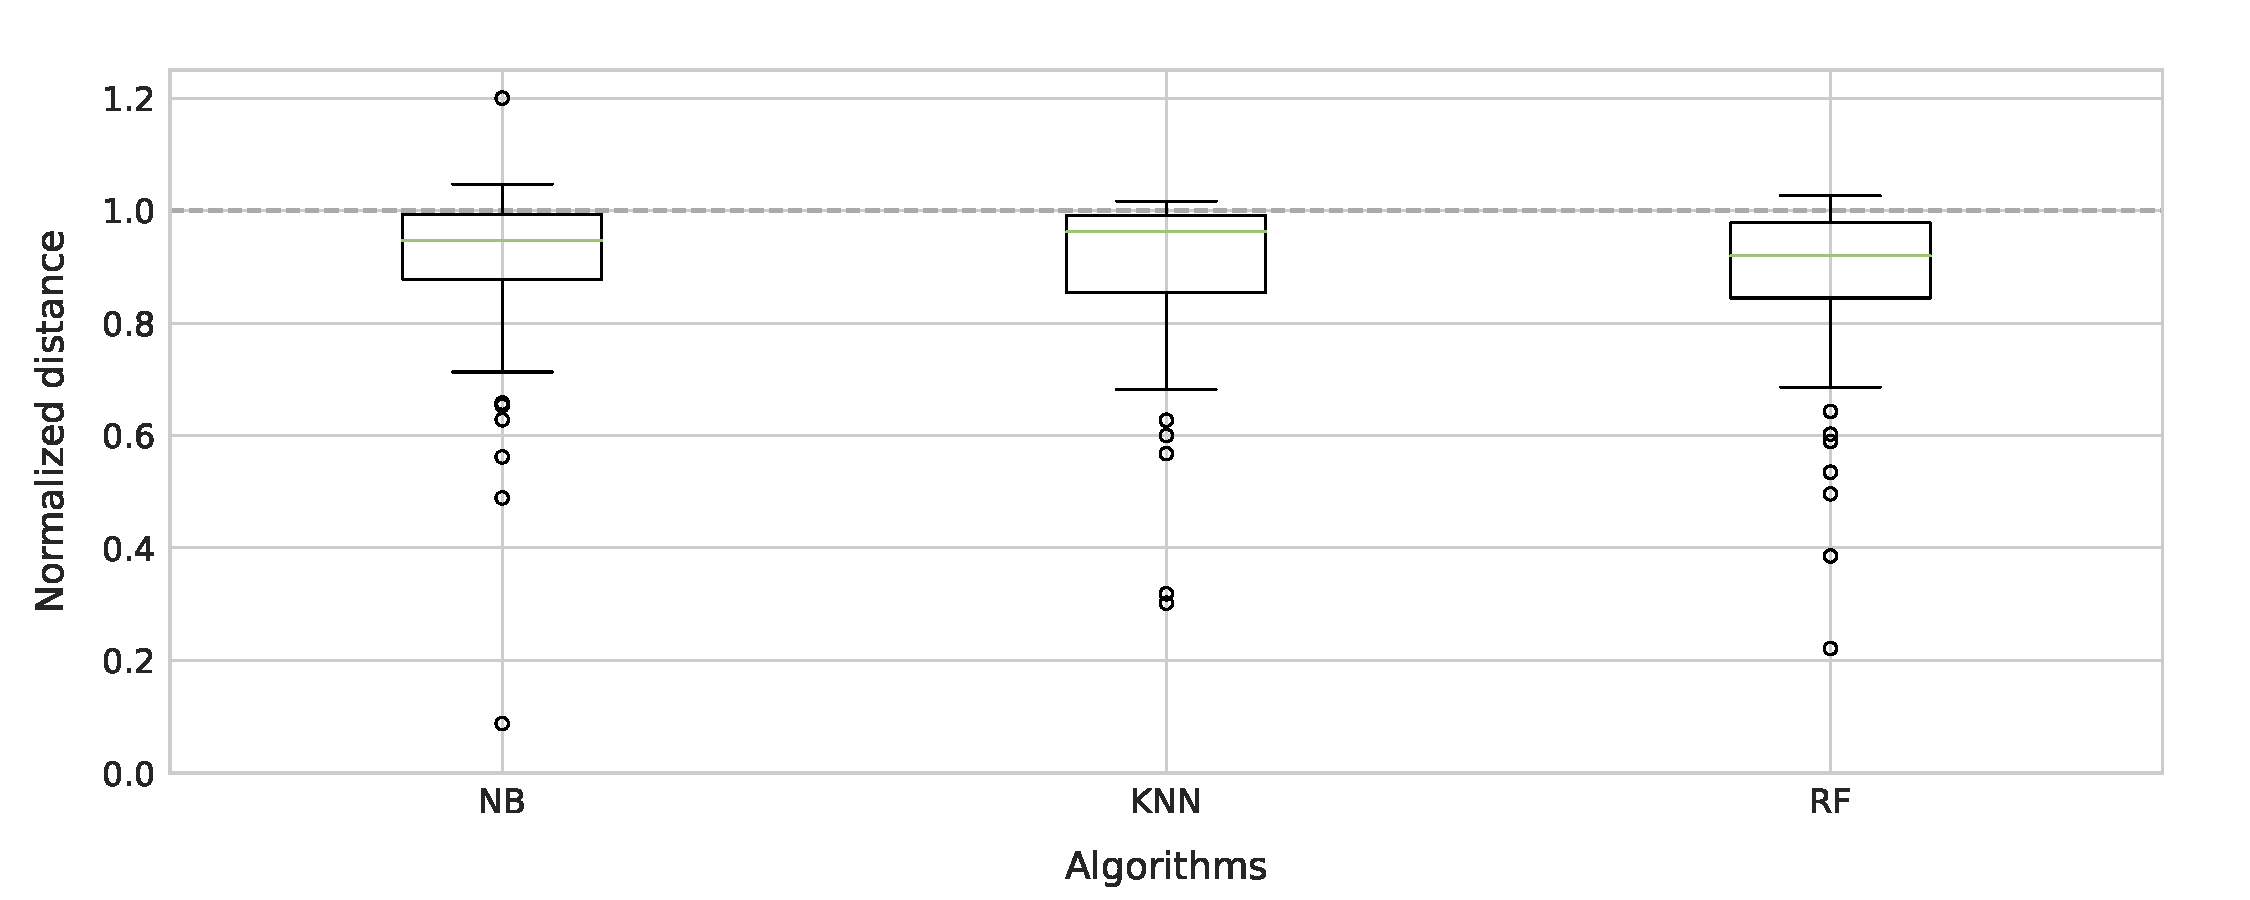
\includegraphics[width=0.7\textwidth]{chapters/data-centric/supervised/img/evaluation2.pdf}
    \caption{Normalized distances between the scores obtained by optimizing our effective prototypes and the ones obtained optimizing the exhaustive set.}
    \label{fig:eval-exhaustive-vs-effective}
\end{figure}

\subsection{Complementing hyper-parameter optimization with pre-processing}
\label{sec:eval-dpso-vs-cash}

\begin{figure*}[!t]
	\centering
	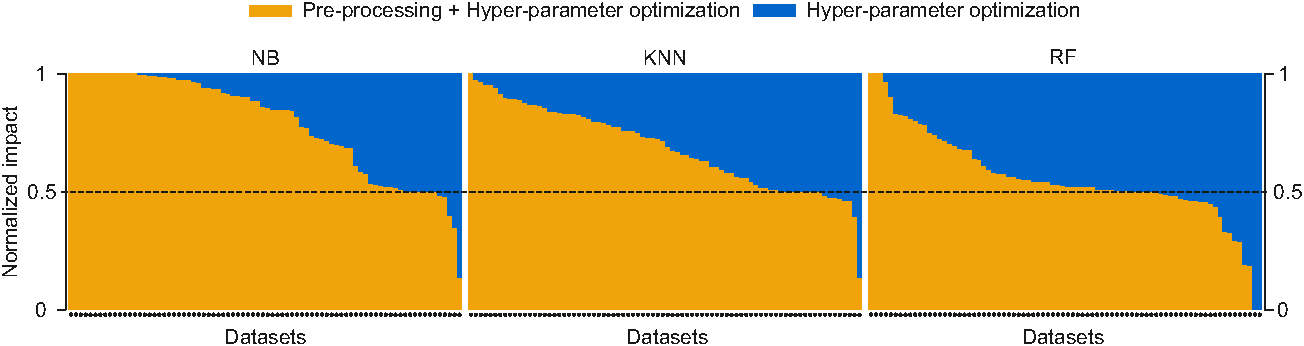
\includegraphics[width=1.0\textwidth]{chapters/data-centric/supervised/img/barplot-10.pdf}
	\caption{The impact of dedicating a portion of the optimization budget to pre-processing compared to using the whole optimization budget for the hyper-parameter optimization.}
	\label{fig:eval-pre-processing-hyper-parameter}
\end{figure*}

We have just shown that our effective pipeline prototypes have similar impact as the exhaustive prototypes. Now we want to compare the impact of effective prototypes against optimizing only the hyper-parameters of the ML algorithm. That is, we want to examine whether dedicating a part of the optimization budget to the pre-processing pipeline impacts more (positively) the results of the analysis, than using the whole budget for the hyper-parameter optimization\footnote{To enable the application of the ML algorithms on all the datasets, whenever required, we apply the necessary transformation (e.g, imputation or encoding).}. 

To this end, for the latter we now dedicate the total optimization budget (i.e., 400 seconds), and for the former, inspired by \cite{Quemy20InfSystems}, we split the budget 50-50 between the pre-processing pipeline optimization and the hyper-parameter optimization (i.e., 200 seconds for the pre-processing, and 200 seconds for the hyper-parameter optimization). The time for the pre-processing is further split among the five different pipeline prototypes (i.e., 40 seconds each).

To compare the results, we calculate the impact using the formulas below, that correspond to the normalized distance from either pre-processing or hyper-parameter optimization to the maximum improvement that can be achieved, regardless of whether pre-processing is applied or not. 

\begin{equation*}
    \text{\textit{pp impact}} = \frac{Acc(d_{e\!f\!f\!ective},a^*) - Acc(d,a)}{max(Acc(d_{e\!f\!f\!ective},a^*),Acc(d,a^*)) - Acc(d,a)}
\end{equation*}

\begin{equation*}
    \text{\textit{hp impact}} = \frac{Acc(d,a^*) - Acc(d,a)}{max(Acc(d_{e\!f\!f\!ective},a^*),Acc(d,a^*)) - Acc(d,a)}
\end{equation*}

where, $Acc(d,a)$ is the baseline accuracy (i.e., predictive accuracy of the algorithm $a$ with default hyper-parameters over the original dataset $d$). $Acc(d_{e\!f\!f\!ective},a^*)$ is the accuracy of the optimized algorithm $a^*$ over the dataset $d_{e\!f\!f\!ective}$ transformed using the optimized instantiation of the effective set of prototypes obtained using our method. Finally,  $Acc(d,a^*)$ is the accuracy of the optimized algorithm $a^*$ (i.e, using the entire budget) over the original dataset $d$.

To obtain relative values that sum to 1, we normalize the impacts dividing them by their sum. For instance, for the pre-processing score we calculate the following:
\begin{equation*}
    \text{\textit{normalized pp impact}} = \frac{\text{\textit{pp impact}}}
    {\text{\textit{pp impact}} + \text{\textit{hp impact}}}
\end{equation*}


We perform the same for the hyper-parameter impact and plot the results obtained for all the algorithms and datasets in Figure~\ref{fig:eval-pre-processing-hyper-parameter}, where each bar represents the results obtained for a single dataset. The different colors represent the impact values of pre-processing and hyper-parameter optimization. 

Observing the bar-charts one can see that (i) dedicating a portion of the budget to pre-processing, brings benefit to the analysis in most of the cases (i.e., $73\%$ of the cases), and (ii) the impact of hyper-parameter optimization, increases with the increase of the number of hyper-parameters of the ML algorithm (e.g., hyper-parameter optimization impacts more RF than NB). Overall, we can conclude that pre-processing is a critical step that once effectively applied may have a high positive impact on the final result of the analysis.


\section{Related work}
\label{sec:relatedwork}
A lot of ongoing research aims at addressing the problem of providing user assistance for the data analytics process.
Specifically, they can be classified into three main categories~\cite{elshawi2019automated}: distributed, cloud-based, and centralized. The first two try to address the problem of Big Data. Thus, clusters of several machines are employed to distribute the workload. On the contrary, this is not a fundamental requirement for centralized solutions. Indeed, the overhead of using a cluster is not worth for relatively small datasets. 
Since our work belongs to the category of centralized solutions, in the following, we provide examples of them.

As already mentioned before, the data analytics process consists of different steps. In general, there is a trend to develop (semi) automatic systems that assist the user in one or many steps altogether. At the beginning, the focus was to provide support exclusively for the learning step (i.e., the CASH problem). Recently however, the direction has shifted towards designing systems that additionally or specifically provide user assistance in the data pre-processing step (i.e., the DPSO problem).

When it comes to data pre-processing, different works have tackled this problem from different perspectives. For instance, there are works that aim to apply pre-processing for the sake of guaranteeing data quality, or enabling data exchange, or even data integration. That is, they consider data pre-processing in isolation or apart from data analysis~\cite{Llunatic13VLDBEnd,BigDansing15SIGMOD,Katara15SIGMOD,Foofah17SIGMOD}. In this, and our related work however, we consider only the works that see pre-processing as an integral part of data analytics and hence apply it for the sake of improving the final result of the analysis.


Finally, there are works that aim at fully automating the data analytics process (i.e., automatically generate data analytics flows), which roughly translates to combining DPSO with CASH, where the border line between the latter two becomes blurry. Nevertheless, we tentatively group the works based on the type of the problem they aim to solve.

\subsection{DPSO}

In DPD \cite{Quemy20InfSystems}, the DPSO problem, as we use it in this work, is formally defined. Authors demonstrate the impact of optimizing the pre-processing pipeline, but considering only a single fixed pipeline prototype. %and only a few datasets. 
However, as we have already seen (Section~
\ref{sec:eval-universal-pipeline}), a single fixed prototype cannot perform best for every dataset. Therefore, we build on top of~\cite{Quemy20InfSystems}, and instead of relying on a fixed prototype, we define a method to generate the right pipeline prototypes to be optimized.

In PRESISTANT~\cite{presistant18CSI,presistant18CAISE,presistant19DKE}, we tackled the problem of recommending pre-processing operators to the non-expert data analyst. The goal, and at the same time the challenge was to identify the pre-processing operators, and rank them in advance, based on their potential impact to the final analysis. However, we did not consider pre-processing pipelines, but only single transformations, expecting that the analyst applies the process iteratively. In this work, we consider sets of transformations and thus study the impact of combining transformations into a pipeline. 

In ActiveClean \cite{ActiveClean16PVLDB}, authors define an algorithm that aims at prioritizing the cleaning of records that are more likely to affect the results of the statistical modeling problems, assuming that the latter belong to the class of convex loss models (i.e., linear regression and SVMs). Hence, instead of recommending the transformations to be applied, the system recommends the subset of data which needs to be cleaned at a given point. The type of pre-processing to be applied is left to the user, assuming that the user is an expert. 

In Learn2Clean~\cite{Berti19WWW}, based on a reinforcement learning technique, for a given dataset, and an ML model, an optimal sequence of operators for pre-processing the data is generated,
such that the quality of the ML model is maximized. Here, similarly to~\cite{Quemy20InfSystems}, the pipeline prototype is fixed in advance. Our work is a step further in that we help to choose the right pipeline prototype, instead of fixing it in advance. 

In Alpine Meadow~\cite{Shang19SIGMOD}, authors follow a similar approach to ours in that they define two steps for the pre-processing phase. One, the so called \textit{logical pipeline plan}, which is roughly equivalent to the \textit{pipeline prototypes} defined in this work, and the second the \textit{physical pipeline plan} which translates to \textit{pipelines} used in this work. The physical plan is generated through a combination of Bayesian optimization, meta-learning, and multi-armed bandits. For the logical plans, they rely on rules but without clear evidence on how they are generated. Moreover, it is not clear whether the logical plan is fixed as in~\cite{Quemy20InfSystems} and if some further adjustment from the user is required. 

\subsection{CASH} The task in solving the CASH problem is to automatically find an optimized instantiation for the hyper-parameters of the ML algorithm. Most of the works use Bayesian optimization methods to tune and optimize them~\cite{Feurer15AutoSklearn,Thornton13AutoWeka,Olson16Tpot}. Since Bayesian optimization is randomized, meta-learning has been used to find a good seed for the search~\cite{Feurer15AAAI}. Most of these works however, only minimally consider the data pre-processing step.
Auto-WEKA~\cite{Thornton13AutoWeka}, based on the Java machine learning library Weka, is the pioneer of the field.
The authors formalized the problem of algorithm selection and their associated hyper-parameter optimization, and solved it in a combined search space. 
Sequential Model-based Algorithm Configuration (SMAC) is used to explore the large search space.

Autostacker~\cite{chen2018autostacker} combines a hierarchical stacking architecture and an evolutionary algorithm (EA).
Stacking is an ensemble method that involves the concatenation of several classifiers, so that the later layers can learn the mistakes that classifiers in the previous layers make.
Even if it brings some benefits, this approach affects the search space: way larger than that of a single classifier.
In a nutshell, such concatenations are randomly generated and then optimized.
The one that achieves the higher predictive accuracy is chosen.
Rather than Bayesian Optimization, to find suitable hyper-parameters, the authors utilize a basic Evolutionary Algorithm.

OBoe~\cite{yang2019oboe} exploits collaborative filtering for AutoML, choosing models that have performed well on similar datasets.
It collects a large number of datasets and applies different ML algorithms (with different hyper-parameters configurations). 
In this way, a matrix of cross-validated errors is built.
Common approaches typically compute dataset meta-features and use them to predict the error of a particular machine learning model, but OBoe works exactly the other way around.
PCA is applied on such a matrix in order to find latent meta-features.
Given a new dataset, some basic algorithms are applied to infer a feature vector (i.e., the value of the latent meta-features).
Finally, the feature vector is leveraged to estimate the cross-validated error of more complex algorithms.

\subsection{DPSO + CASH}
Auto-sklearn~\cite{Feurer15AutoSklearn} is based on the popular Python library scikit-learn.
The authors, inspired by Auto-Weka, address the problem with the Sequential Model-based Algorithm Configuration (SMAC).
Furthermore, they improve the approach by adding a meta-learning phase at the beginning (to warm-start the Bayesian Optimization) and an ensemble technique at the end (to suggests multi-classifiers).
Such a system considers pre-processing transformations to generate end-to-end analytic pipelines. 
Yet, they consider a small set of transformations and also consider a single fixed pipeline prototype. 
Our work in a way is complementary to this, since instead of a priori fixing the prototype, we can construct a potentially optimal one (or a set), and then provide it to the tool for it to be instantiated and further optimized.
TPOT~\cite{Olson16Tpot} is a tree-based pipeline optimization tool using genetic programming while requiring little to no expertise from the user. In TPOT however, they only consider one transformation inside the optimization process (i.e., Feature Engineering).


ML-Plan~\cite{mohr2018ml} uses hierarchical planning, a particular form of AI planning, to propose a solution to both the pre-processing and the modeling phases. 
As in context-free grammars, there are complex tasks (non-terminal symbols) that are derived as long as primitive tasks (terminal symbols) are not obtained.
Typically, standard graph search algorithms (e.g., depth-first search, best-first search, etc.) are employed to solve such problems.
ML-Plan successively creates solutions in a global search instead of changing given solutions in a local search. However, due to the problem constraints, they adopt a randomized best-first search, randomly choosing the solution path.

AutoBazaar~\cite{AutoBazaar} is a Python open-source tool.
Like in ML-Plan~\cite{mohr2018ml}, both pre-processing and modeling phases are covered.
Here the last step of a prototype is the machine learning algorithm.
The approach involves two different steps.
Firstly, a \textit{catalog} proposes a collection of prototypes (with an ML algorithm as last step) based on the task and the dataset itself.
Secondly, the optimization process starts tuning the prototypes until either the time budget is expired or the prototypes are all optimized.
In particular, a \textit{selector} and a \textit{tuner} work in synergy.
The former decides which prototype should be optimized next.
Such a task is treated as a multi-armed bandit problem.
As to the tuner, Bayesian Optimization is chosen.
At the end, the prototype that achieved the higher predictive accuracy is elected.
However, AutoBazaar strictly depends on the catalog.
Such a component memorizes all the possible primitives and supported tasks.
The prototypes are hard-coded for each task.
Thus, it is neither flexible nor maintainable.
If a task is not implemented, the approach cannot suggest a solution.

To summarize, full automation of data analytics has been the ultimate goal of many research works. Yet, such an automation has shown to be computationally expensive, mainly due to the search space involved (i.e., pre-processing and mining operators). Therefore, the usability of these approaches in realistic scenarios is sometimes limited. Our approach of finding a set of effective pipeline prototypes can be seen as complementary to these solutions, since it helps in pruning the large space and guiding the search, hence reducing their cost.

\section{Conclusions and future work}
\label{sec:conclusions}

In this work, we first studied the overall impact of transformations when chained together inside pre-processing prototypes and then delved into examining the impact of instantiating transformations via various operators. As a result, we defined a method that allows to generate effective pre-processing pipelines. That is, pipelines that consist of, (i) compatible pairs of transformations with respect to the framework used,  (ii) meaningful pairs of transformations in terms of general knowledge (best practices), and (iii) promising pairs of transformations that once applied are expected to provide higher overall impact (domain knowledge). 
In addition, via the meta-learning step proposed, we aim to guide the instantiation of transformations in order to facilitate finding better instantiations.

An extensive evaluation on 80 datasets with heterogeneous characteristics, from sample size to feature types, and a set of classification algorithms (i.e., Naive Bayes, Random Forest, K-Nearest Neighbours), showed that our devised pipeline prototypes give promising results. More specifically, we were able to observe that:
\begin{itemize}
    \item [--] The overall impact of optimizing pre-processing is not negligible and it may boost the performance of the overall analytics (e.g., predictive accuracy).
    \item [--] There is no universal pre-processing pipeline prototype that works best for every dataset and algorithm.
    \item [--] With 24 times less time budget, our proposed pipeline prototypes were able to obtain results that were as good as 90\% in the median of the optimal ones found through an exhaustive search.
    \item [--] Dedicating a portion of the time to the pre-processing optimization, instead of dedicating it entirely to hyper-parameter optimization may boost %(have a higher impact on?!) 
    the final result of the analysis. On average, in 73\% of the cases including pre-processing in the optimization, outperformed the results of only optimizing hyper-parameters.
\end{itemize}

The results indicate that pre-processing can boost the performance of the ML algorithm. Hence, it must be considered as an integral part of the data analytics optimization process. 

Finally, previous works have shown the effectiveness of meta-learning for solving the cold start problem~\cite{Feurer15AAAI}, hence as immediate future work, we intend to extend an optimization framework (i.e., HyperOpt) with a complementary meta-learning module that can ease the cold-start problem, facilitating the search for optimal instantiations.